\section{Diversion ratios}\label{sec:04-diversion}

The pricing rule of \cref{sec:04-bertrand} depends on own-price and cross-price derivatives of demand.
Elasticities summarize these derivatives product by product. Diversion ratios summarize them pair by pair:
they record where the customers of a product go when its price rises. This makes them the natural language
for three questions that recur in this book. Which products compete most closely? How does a multi-product
firm price products that cannibalize one another? Which mergers create an incentive to raise prices? This
section defines diversion ratios, rewrites the first-order condition in terms of them, computes them in the
standard demand systems, and lists what they cannot tell us.

\subsection{Definitions and basic properties}\label{sec:04-diversion-def}

We keep the environment of \cref{ass:04-bertrand}. To lighten the notation we write
\[
  \partial_k q_j \equiv \frac{\partial q_j(p)}{\partial p_k}
\]
for the derivative of the demand for product $j$ with respect to the price of product $k$. In this notation
the $(j,k)$ element of $\Delta$ is $\partial_k q_j$. The \emph{cross-price derivative} $\partial_j q_k$ is the
change in the sales of product $k$ when the price of product $j$ rises by one dollar. The \emph{cross-price
elasticity} is $\varepsilon_{kj} = \frac{\partial q_k}{\partial p_j}\frac{p_j}{q_k}$, and the own-price
elasticity is the positive number $\varepsilon_j = -\frac{\partial q_j}{\partial p_j}\frac{p_j}{q_j}$.

\begin{definition}[Diversion ratio]\label{def:04-diversion}
For two inside products $j \neq k$, the \emph{diversion ratio} from $j$ to $k$ is
\begin{equation}\label{eq:04-diversion-def}
  D_{jk} = -\frac{\partial_j q_k}{\partial_j q_j}.
\end{equation}
The \emph{diversion ratio to the outside good} is $D_{j0} = 1 - \sum_{k \ge 1, k \neq j} D_{jk}$, and the
\emph{aggregate diversion ratio} of product $j$ is $\sum_{k \ge 1, k \neq j} D_{jk} = 1 - D_{j0}$.
\end{definition}

The numerator and the denominator of \eqref{eq:04-diversion-def} refer to the same experiment, a small
increase $\dd p_j$ in the price of product $j$ with all other prices fixed. Product $j$ loses
$-\partial_j q_j \, \dd p_j$ units of sales. Product $k$ gains $\partial_j q_k\, \dd p_j$ units. The diversion
ratio is the fraction of the lost units that product $k$ recaptures. Read in reverse, it is the number of
units of $k$ that are lost when $p_j$ falls by enough to sell one more unit of $j$. The first index always
names the product whose price changes. In general $D_{jk} \neq D_{kj}$.

\begin{proposition}[Adding up]\label{prop:04-diversion-adding}
Suppose that each of $M$ consumers buys exactly one unit of one of the options $0, 1, \dots, J$, so that
$\sum_{k=0}^J q_k(p) = M$ for every price vector $p$. Then for every inside product $j$,
\begin{equation}\label{eq:04-diversion-adding}
  \sum_{k \ge 1,\, k \neq j} D_{jk} + D_{j0} = 1, \qquad\text{with}\qquad D_{j0} = -\frac{\partial_j q_0}{\partial_j q_j}.
\end{equation}
If all products, including the outside good, are gross substitutes, every diversion ratio lies in $[0,1]$.
\end{proposition}

\begin{proof}
Differentiate the identity $\sum_{k=0}^J q_k(p) = M$ with respect to $p_j$. The right side does not depend
on prices, so
\[
  \partial_j q_j + \sum_{k \ge 1,\, k \neq j}\partial_j q_k + \partial_j q_0 = 0.
\]
Divide by $-\partial_j q_j > 0$:
\[
  -1 + \sum_{k \ge 1,\, k\neq j}\Bigl(-\frac{\partial_j q_k}{\partial_j q_j}\Bigr) + \Bigl(-\frac{\partial_j q_0}{\partial_j q_j}\Bigr) = 0.
\]
The terms in parentheses are $D_{jk}$ and $-\frac{\partial_j q_0}{\partial_j q_j}$, which gives
\eqref{eq:04-diversion-adding}. Under gross substitutes each term is nonnegative. Nonnegative numbers
that sum to one each lie in $[0,1]$.
\end{proof}

In unit-demand models the residual $D_{j0}$ in \cref{def:04-diversion} is the share of lost customers who
stop buying any inside product. A large $D_{j0}$ then means that the products in the group constrain one
another little. This is why the aggregate diversion ratio appears in market definition (\cref{ch:mergers}).
Some demand systems have no explicit outside option, such as the linear and CES systems of
\cref{sec:04-repcons}. Their quantities need not add up in units, so $D_{j0}$ is only the residual of
\cref{def:04-diversion}. It changes when we rescale the units of one product, and in CES it can be negative.
Reading it as the fraction of $j$'s lost units that the group does not recapture requires units that are
comparable across products.

Diversion ratios and elasticities carry the same information, arranged differently. Write each derivative
in terms of an elasticity:
\[
  \partial_j q_k = \varepsilon_{kj}\frac{q_k}{p_j}, \qquad \partial_j q_j = -\varepsilon_j\frac{q_j}{p_j}.
\]
Substituting into \eqref{eq:04-diversion-def}, the price $p_j$ cancels and
\begin{equation}\label{eq:04-diversion-elast}
  D_{jk} = \frac{\varepsilon_{kj}}{\varepsilon_j}\,\frac{q_k}{q_j}.
\end{equation}
A large cross elasticity does not imply a large diversion ratio. If product $k$ is small, a large percentage
gain for $k$ is a small number of units. Conversely, a large product can capture many of $j$'s customers even
when its own percentage gain is modest.

\casehead{Measurement}
Diversion ratios can be computed from an estimated demand system (\cref{ch:logit,ch:blp}). They can also be
measured more directly, which is a large part of their appeal to antitrust agencies. Firms often track whom
they lose business to, and surveys can ask buyers of $j$ what they would have bought instead
\citep[p.~16]{FarrellShapiro2010}. Natural experiments that remove a product, such as stock-outs, recalls and
exits, reveal where its customers go. In bidding markets the diversion ratio from $j$ to $k$ can be read as
the probability that $k$ is the runner-up when $j$ wins \citep[p.~16]{FarrellShapiro2010}.

These sources do not all measure the same object. \citet{ConlonMortimer2021} view a diversion ratio as a
treatment effect and stress that the size of the price change matters. Second-choice data describe what
happens when product $j$ disappears, which is a price increase to infinity. The pricing incentive in
\eqref{eq:04-foc-diversion} below involves a marginal price change. A mixture of logits shows the
difference. Let consumer types $i$ have distribution $F$, price coefficient $\alpha_i$ and logit choice
probabilities $s_{ij}$, so that $s_j = \int s_{ij}\,\dd F(i)$. Using \eqref{eq:04-logit-derivs} type by type,
the marginal diversion ratio is
\begin{equation}\label{eq:04-diversion-marginal}
  D_{jk} = \frac{\int \alpha_i s_{ij}s_{ik}\,\dd F(i)}{\int \alpha_i s_{ij}(1 - s_{ij})\,\dd F(i)}
         = \int \varpi_i\,\frac{s_{ik}}{1 - s_{ij}}\,\dd F(i),
  \qquad \varpi_i = \frac{\alpha_i s_{ij}(1 - s_{ij})}{\int \alpha_{i'} s_{i'j}(1 - s_{i'j})\,\dd F(i')}.
\end{equation}
When $j$ is removed, a type-$i$ buyer of $j$ moves to $k$ with probability
$\frac{e^{\delta_{ik}}}{\sum_{l \neq j}e^{\delta_{il}}} = \frac{s_{ik}}{1 - s_{ij}}$, where $\delta_{il}$ is the
mean utility of option $l$ for type $i$. Averaging over the buyers of $j$ gives the second-choice diversion
ratio
\begin{equation}\label{eq:04-diversion-secondchoice}
  D^{\mathrm{SC}}_{jk} = \int \tilde\varpi_i\,\frac{s_{ik}}{1 - s_{ij}}\,\dd F(i), \qquad \tilde\varpi_i = \frac{s_{ij}}{s_j}.
\end{equation}
Both are weighted averages of the same type-level ratios $\frac{s_{ik}}{1 - s_{ij}}$. The marginal ratio
weights types by $\alpha_i s_{ij}(1 - s_{ij})$, which is large for price-sensitive consumers near the margin
of buying $j$. The second-choice ratio weights all current buyers of $j$ equally. With one type both reduce
to the logit formula $\frac{s_k}{1 - s_j}$. With heterogeneous consumers they differ, and a survey answer
needs a model before it can be plugged into a pricing formula.

\subsection{The first-order condition in diversion form}\label{sec:04-diversion-foc}

The multi-product first-order condition \eqref{eq:04-foc-scalar} can be rewritten so that diversion ratios
appear explicitly. For firm $f$ and a product $j \in \mathcal{J}_f$ the condition reads
\[
  q_j + \sum_{k \in \mathcal{J}_f}(p_k - mc_k)\,\partial_j q_k = 0.
\]
We first split off the term $k = j$:
\[
  q_j + (p_j - mc_j)\,\partial_j q_j + \sum_{k \in \mathcal{J}_f\setminus\{j\}}(p_k - mc_k)\,\partial_j q_k = 0.
\]
Next we divide by $\partial_j q_j < 0$:
\[
  \frac{q_j}{\partial_j q_j} + (p_j - mc_j) + \sum_{k \in \mathcal{J}_f\setminus\{j\}}(p_k - mc_k)\frac{\partial_j q_k}{\partial_j q_j} = 0.
\]
Solving for $p_j$ gives
\[
  p_j = mc_j - \frac{q_j}{\partial_j q_j} - \sum_{k \in \mathcal{J}_f\setminus\{j\}}(p_k - mc_k)\frac{\partial_j q_k}{\partial_j q_j}.
\]
Finally, $-\frac{\partial_j q_k}{\partial_j q_j} = D_{jk}$ by \eqref{eq:04-diversion-def}, so
\begin{equation}\label{eq:04-foc-diversion}
  p_j = mc_j + \frac{q_j}{-\partial_j q_j} + \sum_{k \in \mathcal{J}_f\setminus\{j\}} D_{jk}\,(p_k - mc_k).
\end{equation}

The price of product $j$ has three parts. The first is marginal cost. The second is the markup a
single-product firm would charge, the reciprocal of the absolute semi-elasticity of $q_j$. The third is the
\emph{value of diverted sales}: each unit of $j$'s lost sales that moves to a sibling product $k$ earns the
firm the margin $p_k - mc_k$. This term is an opportunity cost of selling $j$, because every extra unit of $j$
cannibalizes $D_{jk}$ units of $k$. Define the \emph{effective marginal cost}
$\widetilde{mc}_j = mc_j + \sum_{k \in \mathcal{J}_f\setminus\{j\}}D_{jk}(p_k - mc_k)$. Then
\eqref{eq:04-foc-diversion} becomes $p_j - \widetilde{mc}_j = \frac{q_j}{-\partial_j q_j}$, and dividing by
$p_j$,
\[
  \frac{p_j - \widetilde{mc}_j}{p_j} = \frac{1}{\varepsilon_j}.
\]
A multi-product firm prices each product by the inverse elasticity rule, applied to an effective marginal cost
that includes the value of diverted sales. The 2010 US Horizontal Merger Guidelines use this phrase for the units
diverted to a product multiplied by that product's margin \citep[Section 6.1, p.~21]{USDOJFTC2010}. The term in
\eqref{eq:04-foc-diversion} is this value per unit of lost sales of $j$.

Stacking \eqref{eq:04-foc-diversion} over products gives a compact matrix version. Let
$m^{\mathrm{s}}_j = \frac{q_j}{-\partial_j q_j}$ be the single-product markup, with vector $m^{\mathrm{s}}$, let
$m = p - mc$, and let $\mathcal{D}$ be the $J \times J$ \emph{diversion matrix} with $\mathcal{D}_{jk} = D_{jk}$ for
$k \neq j$ and zeros on the diagonal. Since $\Omega_{jk} = 1$ exactly when $j$ and $k$ have the same owner,
\begin{equation}\label{eq:04-markup-diversion}
  m = m^{\mathrm{s}} + (\Omega \odot \mathcal{D})\,m, \qquad\text{so}\qquad m = (I - \Omega \odot \mathcal{D})^{-1} m^{\mathrm{s}}.
\end{equation}
This is the stacked first-order condition \eqref{eq:04-foc-matrix} with row $j$ divided by $-\partial_j q_j$, and its
solution coincides with the markup equation \eqref{eq:04-markup}.

\begin{remark}\label{rem:04-diversion-positive}
Equation \eqref{eq:04-markup-diversion} gives a short proof that markups are positive. Suppose that every
outside diversion ratio is positive, $D_{j0} > 0$. Row $j$ of $\Omega\odot\mathcal{D}$ has nonnegative
entries that sum to at most $\sum_{k \neq j}D_{jk} = 1 - D_{j0} < 1$. The sup-norm of
$\Omega\odot\mathcal{D}$ is therefore below one, and the Neumann series
$(I - \Omega\odot\mathcal{D})^{-1} = \sum_{n=0}^\infty(\Omega\odot\mathcal{D})^n$ converges to a matrix with
nonnegative entries and diagonal entries of at least one. Hence $m \ge m^{\mathrm{s}} > 0$ element by element. Every product of a
multi-product firm carries at least its single-product markup, in line with \cref{prop:04-markup-positive}.
\end{remark}

Two examples from \cref{sec:04-bertrand} show the formula at work. In the linear duopoly of
\cref{ex:04-linear-duopoly}, $\partial_1 q_1 = -b$ and $\partial_1 q_2 = d$, so $D_{12} = \frac{d}{b} \equiv D$.
For a joint owner, \eqref{eq:04-foc-diversion} reads $m_1 = \frac{q_1}{b} + D\,m_2$. At a symmetric
solution $m(1 - D) = \frac{q}{b}$ with $q = a - (b - d)(c + m)$. Multiplying by $b$ and using
$b(1 - D) = b - d$,
\[
  (b - d)\,m = a - (b - d)c - (b - d)m \quad\Longrightarrow\quad m^J = \frac{a - (b - d)c}{2(b - d)},
\]
the joint-owner markup found in \cref{ex:04-linear-duopoly}. In the multi-product logit model the
derivatives \eqref{eq:04-logit-derivs} give $D_{jk} = \frac{s_k}{1 - s_j}$ and
$m^{\mathrm{s}}_j = \frac{1}{\alpha(1 - s_j)}$. With the common markup $m_f$ of \cref{prop:04-logit-markup},
\eqref{eq:04-foc-diversion} becomes
\[
  m_f = \frac{1}{\alpha(1 - s_j)} + \frac{S_f - s_j}{1 - s_j}\,m_f
  \quad\Longrightarrow\quad m_f\,\frac{1 - S_f}{1 - s_j} = \frac{1}{\alpha(1 - s_j)}
  \quad\Longrightarrow\quad m_f = \frac{1}{\alpha(1 - S_f)},
\]
where $S_f = \sum_{k \in \mathcal{J}_f}s_k$. The firm's combined share enters because the recaptured
fraction $\frac{S_f - s_j}{1 - s_j}$ grows with the shares of the sibling products.

\subsection{Why diversion governs the unilateral effects of mergers}\label{sec:04-diversion-merger}

Equation \eqref{eq:04-foc-diversion} explains why diversion ratios dominate the analysis of
\emph{unilateral effects}. These are the price effects of a merger that arise because the merged firm
internalizes competition between its own products, with the conduct of rivals unchanged. A merger adds the
acquired products to $\mathcal{J}_f\setminus\{j\}$ and so adds terms $D_{jk}(p_k - mc_k)$ to the effective marginal
cost of product $j$. The size of these terms depends on how close the merging products are as substitutes. The
merging firms' shares of a predefined market play no direct role.

Consider two single-product Bertrand firms, $A$ selling product 1 and $B$ selling product 2, with constant
marginal costs. Before the merger, firm $A$'s first-order condition is
$q_1 + (p_1 - mc_1)\,\partial_1 q_1 = 0$. After the merger, one owner maximizes $\pi_1 + \pi_2$. Evaluated at
the pre-merger prices, the derivative of joint profit with respect to $p_1$ is
\[
  \frac{\partial(\pi_1 + \pi_2)}{\partial p_1}
  = \underbrace{q_1 + (p_1 - mc_1)\,\partial_1 q_1}_{=\,0 \text{ before the merger}} + (p_2 - mc_2)\,\partial_1 q_2
  = (p_2 - mc_2)\,\partial_1 q_2 > 0.
\]
The merged firm wants to raise $p_1$. Dividing by $-\partial_1 q_1 > 0$ measures this incentive per unit of
product 1's lost sales. The result, $D_{12}(p_2 - mc_2)$, is the increase in the effective marginal cost of
product 1. \citet[p.~9]{FarrellShapiro2010} interpret it as a ``first-round tax'' that the merged firm's
headquarters would levy on division $A$ to make it internalize the sales it takes from division $B$.

A merger can also lower marginal costs. Let $E_1$ be the proportional reduction in the marginal cost of product
1, so that the merger saves $E_1 mc_1$ per unit. The symbol $E_1$ is unrelated to the logit aggregate $E_f$ of
\cref{sec:04-bertrand-logit}. The \emph{upward pricing pressure} (UPP) on product 1 is
\begin{equation}\label{eq:04-upp}
  \mathit{UPP}_1 = D_{12}(p_2 - mc_2) - E_1\,mc_1,
\end{equation}
evaluated at pre-merger prices and margins. \citet[p.~12, inequality (1)]{FarrellShapiro2010} propose to
presume harm when $\mathit{UPP}_1 > 0$. In the symmetric case, with equal prices $p$, costs $mc$, diversion
ratios $D$ and efficiencies $E$, the condition divides through by $p - mc$ to give
\[
  D > E\,\frac{mc}{p - mc}.
\]
This is their inequality (2), which they state in terms of the relative margin $\frac{p - mc}{p}$. They use $E = 0.1$ as an illustrative default
\citep[p.~10]{FarrellShapiro2010}. With a Lerner index of $\frac{1}{3}$ we have $\frac{mc}{p - mc} = 2$, and the
merger is flagged when $D > 0.2$.

Condition \eqref{eq:04-upp} credits an efficiency to product 1 only. Suppose that the merger also lowers the
marginal cost of product 2 by the fraction $E_2$. Each unit diverted to product 2 then earns the margin
$p_2 - (1 - E_2)mc_2 = (p_2 - mc_2) + E_2\,mc_2$, which is larger even at unchanged prices. At pre-merger prices
the derivative of joint profit with respect to $p_1$, divided by $-\partial_1 q_1$, becomes
\[
  D_{12}\big[(p_2 - mc_2) + E_2\,mc_2\big] - E_1\,mc_1.
\]
In the symmetric case with $E_1 = E_2 = E$ it is positive exactly when $D(p - mc) > (1 - D)E\,mc$, that is, when
$\frac{D}{1 - D} > E\frac{mc}{p - mc}$ \citep[p.~14, inequality (4)]{FarrellShapiro2010}. At equality the
pre-merger prices satisfy both post-merger first-order conditions. The common efficiency $E$ then equals the
compensating marginal-cost reduction of \citet{Werden1996}, which leaves both prices unchanged. Farrell and
Shapiro obtain the general version, their inequality (3), by solving these two markup equations simultaneously.
With the same numbers the condition reads $\frac{D}{1 - D} > 0.2$, so the threshold falls to
$D > \frac{1}{6} \approx 0.167$. Their footnote 35 reports both thresholds, 20 and 16.7 percent. It also notes
that the symmetric condition is equivalent to equation (6) of \citet{Werden1996}. The responses of the two prices
to each other after the merger are a separate feedback. When $p_2$ rises, the margin on diverted sales grows
further and adds to the pricing pressure on product 1 \citep[p.~13]{FarrellShapiro2010}. This feedback changes
the size of the price increase but leaves the threshold unchanged. At the threshold the pre-merger prices already
satisfy both post-merger first-order conditions, so no price moves.

The \emph{gross upward pricing pressure index} (GUPPI) scales the cannibalization term by the price of the product
under study:
\begin{equation}\label{eq:04-guppi}
  \mathit{GUPPI}_1 = \frac{D_{12}(p_2 - mc_2)}{p_1} = D_{12}\,\frac{p_2 - mc_2}{p_2}\,\frac{p_2}{p_1}.
\end{equation}
For example, $D_{12} = 0.2$, a margin of 40 percent on product 2 and equal prices give
\[
  \mathit{GUPPI}_1 = 0.2 \times 0.4 \times 1 = 0.08.
\]
The merger raises the effective marginal cost of product 1 by 8 percent of its price. UPP and GUPPI need
only diversion ratios and margins, and no full demand system. \citet[p.~12, Proposition 1]{FarrellShapiro2010}
show that net upward pricing pressure on both products, with no more than the default efficiencies, implies
that both prices rise. A full merger simulation instead solves the post-merger first-order conditions
$q + (\Omega^{post}\odot\Delta^\top)(p - mc) = 0$ with recovered marginal costs (\cref{sec:04-counterfactuals}).
The derivation with efficiencies, the role of pass-through, the GUPPI thresholds used in practice and
applications are in \cref{ch:mergers}.

\begin{example}[From UPP to price effects in the linear duopoly]\label{ex:04-upp-linear}
The linear duopoly of \cref{ex:04-linear-duopoly} shows how a diversion-based pricing pressure translates into a
price change. Before the merger each markup is $m^N = \frac{a - (b - d)c}{2b - d}$. After it, each markup is
$m^J$, and the ratio is
\[
  \frac{m^J}{m^N} = \frac{2b - d}{2(b - d)} = \frac{2 - D}{2 - 2D}, \qquad D = \frac{d}{b}.
\]
The ratio equals 1.056, 1.167, 1.5 and 2.5 for $D = 0.1$, $0.25$, $0.5$ and $0.75$. In levels,
\[
  m^J - m^N = m^N\Bigl(\frac{2 - D}{2 - 2D} - 1\Bigr) = \frac{D\,m^N}{2(1 - D)}.
\]
Without efficiencies the pre-merger UPP on each product is $D\,m^N$, so the price change is
$\frac{1}{2(1 - D)}$ times the UPP. The factor arises in three rounds. Holding the rival's price fixed, a firm
facing linear demand passes through one half of a cost increase, since its best response
$\frac{a + b(c + t) + d p_k}{2b}$ rises by $\frac{t}{2}$ for a cost increase $t$. If both products bear the
tax $t$ and both prices adjust, the symmetric equilibrium price $\frac{a + b(c + t)}{2b - d}$ rises by
$\frac{t}{2 - D}$. If the tax is then recomputed at the new margins, $t = D(m^N + \Delta p)$. Solving
$\Delta p\,(2 - D) = D(m^N + \Delta p)$ gives $\Delta p = \frac{D\,m^N}{2 - 2D}$, the full effect. The three
rounds follow the iterative procedure of \citet[p.~9]{FarrellShapiro2010}. We impose the internal taxes, let the
oligopoly re-equilibrate, re-calculate the taxes at the new prices and outputs, and repeat these steps until
convergence. Their footnote 24 adds that with strategic complements each round raises prices, so with constant
costs and diversion ratios the taxes rise from round to round. With $a = 10$, $b = 2$,
$d = 1$ and $c = 1$, we have $m^N = 3$, $D = \frac{1}{2}$ and $\mathit{UPP} = 1.5$. The price rises from 4 to
5.5, by exactly the UPP, because $\frac{1}{2(1 - D)} = 1$ when $D = \frac{1}{2}$.
\end{example}

\subsection{Diversion in standard demand systems}\label{sec:04-diversion-systems}

Each demand system used in practice implies a pattern of diversion. Often the pattern is imposed by the
functional form, which is worth knowing before a system is used to evaluate mergers.

\casehead{Logit}
With logit shares, \eqref{eq:04-logit-derivs} gives $\partial_j s_j = -\alpha s_j(1 - s_j)$,
$\partial_j s_k = \alpha s_j s_k$ and $\partial_j s_0 = \alpha s_j s_0$. Hence
\begin{equation}\label{eq:04-diversion-logit}
  D_{jk} = \frac{\alpha s_j s_k}{\alpha s_j(1 - s_j)} = \frac{s_k}{1 - s_j}, \qquad D_{j0} = \frac{s_0}{1 - s_j}.
\end{equation}
Customers who leave $j$ spread over the remaining options in proportion to their shares. A product similar to
$j$ and a product very different from it receive the same diversion if they have the same share. This is the
independence of irrelevant alternatives property (\cref{ch:logit}). It also means that a logit-based UPP adds
no information beyond shares and margins.

\casehead{CES}
Consider the CES system of \cref{sec:04-repcons} with elasticity of substitution $\sigma > 1$. This $\sigma$ is
unrelated to the nesting parameter. Demand is $q_j = \frac{p_j^{-\sigma}}{\sum_k p_k^{1-\sigma}}\,y$, with income $y$
and expenditure shares $s_j = \frac{p_jq_j}{y}$. The quantity diversion ratio is
\begin{equation}\label{eq:04-diversion-ces}
  D_{jk} = \frac{(\sigma - 1)\,p_j\,q_k}{y\,[\sigma - (\sigma - 1)s_j]} = \frac{(\sigma - 1)\,s_k}{\sigma - (\sigma - 1)s_j}\,\frac{p_j}{p_k},
\end{equation}
which \cref{prop:04-ces} derives from the CES elasticities. Diversion is proportional to the quantity $q_k$,
again with no role for similarity.

\casehead{Linear demand}
If $q = a + Ap$ for a vector $a$ and a $J \times J$ matrix $A$, then $\partial_j q_k = A_{kj}$ and
$D_{jk} = -\frac{A_{kj}}{A_{jj}}$. Diversion is constant, and in the symmetric duopoly it equals
$\frac{d}{b}$. A linear system can represent any pattern of diversion at one point, at the cost of $J^2$
price parameters (\cref{sec:04-spaces}).

\casehead{Nested logit}
Group the inside products into nests and let $\sigma^{\mathrm{NL}} \in [0,1)$ be the nesting parameter of
\cref{ch:logit}, written with a superscript in this section to avoid a clash with the CES elasticity. Let
$s_{j\mid g}$ be the share of product $j$ within its nest $g$ and $s_g$ the share of the nest. We use the form
of \citet{Berry1994}, and \cref{ch:logit} derives the share derivatives. With respect to $p_j$ they are
\[
  \partial_j s_j = -\frac{\alpha s_j\bigl[1 - \sigma^{\mathrm{NL}} s_{j\mid g} - (1 - \sigma^{\mathrm{NL}})s_j\bigr]}{1 - \sigma^{\mathrm{NL}}},
  \qquad
  \partial_j s_k = \frac{\alpha s_k\bigl[\sigma^{\mathrm{NL}} s_{j\mid g} + (1 - \sigma^{\mathrm{NL}})s_j\bigr]}{1 - \sigma^{\mathrm{NL}}}
\]
for $k$ in the nest of $j$, and $\partial_j s_k = \alpha s_k s_j$ for $k$ in another nest or $k = 0$. Taking ratios
and using $s_k = s_{k\mid g}s_g$ and $s_j = s_{j\mid g}s_g$,
\begin{equation}\label{eq:04-diversion-nl}
  D_{jk} =
  \begin{cases}
    \displaystyle\frac{s_{k\mid g}\bigl[\sigma^{\mathrm{NL}} + (1 - \sigma^{\mathrm{NL}})s_g\bigr]}{1 - \sigma^{\mathrm{NL}}s_{j\mid g} - (1 - \sigma^{\mathrm{NL}})s_j} & \text{if $k$ is in the nest of $j$,}\\[3ex]
    \displaystyle\frac{(1 - \sigma^{\mathrm{NL}})\,s_k}{1 - \sigma^{\mathrm{NL}}s_{j\mid g} - (1 - \sigma^{\mathrm{NL}})s_j} & \text{otherwise, including $k = 0$.}
  \end{cases}
\end{equation}
At $\sigma^{\mathrm{NL}} = 0$ both lines reduce to \eqref{eq:04-diversion-logit}. As
$\sigma^{\mathrm{NL}}$ approaches one, diversion outside the nest vanishes and the within-nest ratio approaches
$\frac{s_{k\mid g}}{1 - s_{j\mid g}}$. Diversion concentrates within the nest.

\Cref{fig:04-diversion} shows how much this matters. Four inside products sit in two nests, $\{1, 2\}$ and
$\{3, 4\}$. All prices equal 1 and the price coefficient equals 1. For each value of the nesting parameter we
set a common mean utility so that every inside share is 0.15 and the outside share is 0.40. Shares, prices and
margins are therefore identical across the four models. Under logit, the diversion from product 1 is 0.1765 to
each rival and 0.4706 to the outside good. With $\sigma^{\mathrm{NL}} = 0.5$ the diversion to product 2 is
0.4815, against 0.1111 to products 3 and 4 and 0.2963 to the outside good. With $\sigma^{\mathrm{NL}} = 0.7$ the
values are 0.6529, 0.0744, 0.0744 and 0.1983. With $\sigma^{\mathrm{NL}} = 0.9$ they are 0.8692, 0.0280, 0.0280
and 0.0748. Each row sums to one, as \cref{prop:04-diversion-adding} requires. For given margins, the GUPPI of a
merger between products 1 and 2 is 3.7 times larger under the nested logit with $\sigma^{\mathrm{NL}} = 0.7$
than under the logit ($\frac{0.6529}{0.1765} = 3.70$). Shares alone cannot distinguish these markets.

\begin{figure}[htbp]
  \centering
  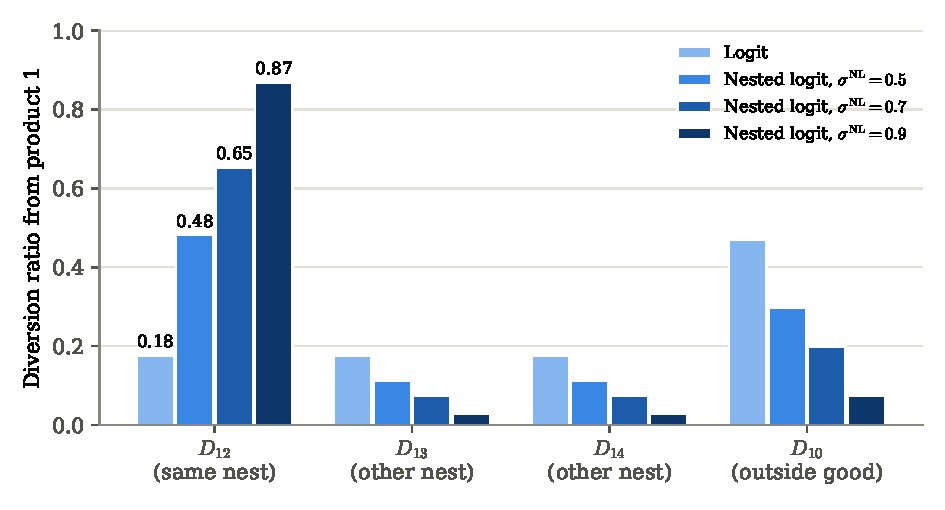
\includegraphics[width=0.95\textwidth]{figures/ch04/diversion_nl.pdf}
  \caption{Diversion ratios from product 1 in four demand models with identical shares. Products 1 and 2 form
  one nest and products 3 and 4 the other. Every inside share is 0.15 and the outside share is 0.40. The logit
  spreads lost sales in proportion to shares. The nested logit sends most of them to the other product in the
  same nest, more so as $\sigma^{\mathrm{NL}}$ rises. Computed with \texttt{figures/ch04/src/diversion\_nl.py}.}
  \label{fig:04-diversion}
\end{figure}

\subsection{What diversion ratios do not tell us}\label{sec:04-diversion-limits}

Diversion ratios are local. They are derivatives evaluated at current prices, and except under linear demand
they change when prices change. A merger moves prices, so diversion at the post-merger prices differs from the
pre-merger value that enters UPP. \Cref{ex:04-upp-linear} shows that even with constant diversion the full
price effect differs from UPP by a factor that depends on $D$.

Diversion ratios give the direction of the pricing incentive. The size of the price change also requires
pass-through, which depends on the curvature of demand (\cref{prop:04-passthrough}, \cref{ch:theory}). For a
single-product firm facing a fixed rival price, pass-through is $\frac{1}{2}$ with linear demand, $1 - s_j$
with logit demand and $\frac{\varepsilon}{\varepsilon - 1} > 1$ with constant-elasticity demand. The same UPP
can therefore produce very different price increases. \citet[Section 3]{FarrellShapiro2010} use this point to
argue that a screen should rely on the sign of pricing pressure, leaving magnitudes to a later stage.

Diversion is directional. When $\Delta$ is symmetric, \eqref{eq:04-diversion-def} implies
$-D_{12}\,\partial_1 q_1 = \partial_1 q_2 = \partial_2 q_1 = -D_{21}\,\partial_2 q_2$, so
$D_{21} = D_{12}\frac{\partial_1 q_1}{\partial_2 q_2}$. Under logit $D_{12} = \frac{s_2}{1 - s_1}$ and
$D_{21} = \frac{s_1}{1 - s_2}$: diversion from a small product to a large one exceeds diversion in the
reverse direction. A merger between a large and a small firm thus creates more pressure on the small firm's
price, for given margins.

Finally, diversion ratios describe demand for a fixed set of products and fixed non-price attributes. They are
silent about entry, repositioning and changes in quality after a merger (\cref{ch:mergers}). When diversion
comes from a demand system rather than from direct evidence, it inherits the system's restrictions. Under
logit, ``measured'' diversion restates an assumption about substitution.

\section{Existence, uniqueness and multiplicity of price equilibria}\label{sec:04-existence}

The pricing rules of \cref{sec:04-bertrand,sec:04-diversion} are first-order conditions. They describe an
equilibrium only if an equilibrium exists and if each firm's first-order condition identifies a global profit
maximum. They predict a single outcome only if the equilibrium is unique. This section asks when these
properties hold. We first explain why existence is a problem in price games with differentiated products. Next
we give conditions on demand that make profit quasi-concave and present the existence theorem of
\citet{CaplinNalebuff1991}. Finally we prove uniqueness for the logit model with any ownership structure and
construct a simple market with two equilibria. Throughout we take the set of products and their characteristics
as given. This is the first of the two branches of theory described in \cref{sec:04-why-division}, and product
choice waits until \cref{sec:04-location}.

\subsection{The existence problem}\label{sec:04-existence-problem}

Consider $F$ firms. Firm $f$ chooses the prices $p_{\mathcal{J}_f}$ of its products from a compact box
$P_f = \prod_{j \in \mathcal{J}_f}[\underline{p}_j, \bar{p}_j]$ and earns $\pi_f(p)$. A \emph{pure-strategy
Bertrand-Nash equilibrium} is a fixed point of the best-response correspondence
$BR(p) = \prod_f BR_f(p_{-\mathcal{J}_f})$, where
$BR_f(p_{-\mathcal{J}_f}) = \argmax_{p_{\mathcal{J}_f} \in P_f}\pi_f(p_{\mathcal{J}_f}, p_{-\mathcal{J}_f})$.
The standard tool is \emph{Kakutani's fixed-point theorem}. A correspondence from a nonempty, compact, convex
subset of $\R^J$ into itself has a fixed point if it has a closed graph and nonempty convex values.

Two of these requirements are usually easy. Berge's maximum theorem concerns a continuous function of a choice
variable and a parameter, maximized over a fixed compact set. It says that the maximizers, as a correspondence of
the parameter, have nonempty compact values and a closed graph. If demand is continuous, profit is continuous, and
the theorem applies to each firm's best response. The difficulty is convexity. The best-response set
is convex when $\pi_f$ is \emph{quasi-concave} in the firm's own prices, that is, when its upper contour sets
are convex. Without restrictions on demand, quasi-concavity can fail. A firm may prefer either a high price
aimed at a small group of consumers for whom its product is well positioned or a low price aimed at the mass
market. Both can dominate every intermediate price \citep[p.~2]{CaplinNalebuff1991}. The best response then
jumps between two prices, and the jump can leave the best-response map without a fixed point.
\Cref{ex:04-multiple-eq} below builds such a profit function. Here and throughout the chapter, page, proposition,
theorem, example and footnote numbers for \citet{CaplinNalebuff1991} refer to the version we checked, Cowles
Foundation Discussion Paper 937 (February 1990). The published article may number them differently.

Continuity can fail as well. In Hotelling's model with linear transport costs, a firm that undercuts its rival
by more than the transport cost between them captures the rival's entire market, so demand jumps.
\citet{DAspremontGabszewiczThisse1979} showed that this discontinuity rules out a pure-strategy price
equilibrium when the firms are close together (\cref{sec:04-location}). Mixed-strategy equilibria exist in
such discontinuous games \citep{DasguptaMaskin1986}, and \citet{OsbornePitchik1987} computed them for
Hotelling's model. Their complexity, however, rules out the comparative statics that applications need
\citep[p.~2]{CaplinNalebuff1991}.

Before \citet{CaplinNalebuff1991}, positive results came from special models in which demand is concave in own
price or log price \citep{GabszewiczThisse1979,ShakedSutton1982,Lane1980,Hauser1988,Economides1989}. These
models are one-dimensional and have consumers distributed uniformly over the market. We will see below that
concavity of demand is too strong a condition to go further.

\subsection{Sufficient conditions on demand*}\label{sec:04-existence-demand}

This subsection collects conditions on a firm's residual demand that make its profit quasi-concave in own price.
Consider a single-product firm with constant marginal cost $c$. Fix the rivals' prices and write $q(p)$ for its
residual demand, assumed nonincreasing in its own price $p$. Let $\bar p$ be the price at which demand reaches
zero, possibly $+\infty$, so that $q > 0$ exactly on $(-\infty, \bar p)$. Profit is $\pi(p) = (p - c)\,q(p)$.

Prices below cost never matter for quasi-concavity. For $p < c$ profit is nonpositive and nondecreasing,
because a higher price reduces both sales and the loss per unit. Formally, where $q$ is differentiable,
$\pi'(p) = q(p) + (p - c)q'(p) \ge 0$ for $p < c$, since $q \ge 0$, $p - c < 0$ and $q' \le 0$. Every result
below therefore concerns prices $p \ge c$.

\begin{lemma}[Log-concave demand]\label{lem:04-logconcave}
If $\ln q$ is concave on $(c, \bar p)$, then $\pi$ is quasi-concave in $p$, and the set of profit-maximizing
prices, when nonempty, is a closed interval. If $\ln q$ is strictly concave there, the maximizer is unique.
\end{lemma}

\begin{proof}
On $(c, \bar p)$ profit is positive and
\[
  \ln \pi(p) = \ln(p - c) + \ln q(p).
\]
The first term is concave in $p$ and the second is concave by assumption. A sum of concave functions is
concave, so $\pi$ is log-concave on $(c, \bar p)$. A log-concave function is quasi-concave, because its upper
contour sets are those of the concave function $\ln\pi$. Outside $(c, \bar p)$ profit is nonpositive, and it is
nondecreasing below $c$. Hence for any $t > 0$ the upper contour set $\{p : \pi(p) \ge t\}$ is a subset of
$(c, \bar p)$ and an interval. For $t \le 0$ it contains every price above $c$, and with the prices below $c$ at
which $\pi \ge t$ it forms a half-line. All upper contour sets are intervals, which is quasi-concavity. If a maximum exists
and $q$ is positive somewhere above $c$, the maximum is positive, so the argmax is an upper contour set of the concave function
$\ln\pi$, a closed interval. Strict concavity of $\ln q$ makes $\ln\pi$ strictly concave, so the maximizer is
unique.
\end{proof}

The next condition is weaker. It requires only that $\frac{1}{q}$ be convex.

\begin{lemma}[Convex reciprocal demand]\label{lem:04-recip}
If $\frac{1}{q}$ is convex on $(-\infty, \bar p)$, then $\pi$ is quasi-concave in $p$
\citep[Proposition 3]{CaplinNalebuff1991}.
\end{lemma}

\begin{proof}
We follow \citet[p.~29]{CaplinNalebuff1991}.
Suppose $\pi$ is not quasi-concave. Then there are prices $p_0 < p_1$ and $\lambda \in (0,1)$ such that, with
$p_\lambda = \lambda p_0 + (1 - \lambda)p_1$,
\[
  \pi(p_0) > \pi(p_\lambda) \qquad\text{and}\qquad \pi(p_1) > \pi(p_\lambda).
\]
By the argument above, $p_0 \ge c$, since otherwise $p_\lambda$ would earn at least as much as $p_0$. Hence
$p_\lambda > c$. If $q(p_1) = 0$, then $\pi(p_1) = 0 > \pi(p_\lambda)$ requires $p_\lambda < c$, a contradiction.
So $q(p_1) > 0$, and because $q$ is nonincreasing, $q(p_0) \ge q(p_\lambda) \ge q(p_1) > 0$. Divide the first
inequality by $q(p_0)q(p_\lambda)$ and the second by $q(p_1)q(p_\lambda)$:
\[
  \frac{p_0 - c}{q(p_\lambda)} > \frac{p_\lambda - c}{q(p_0)}, \qquad \frac{p_1 - c}{q(p_\lambda)} > \frac{p_\lambda - c}{q(p_1)}.
\]
Multiply the first by $\lambda$, the second by $1 - \lambda$, and add. The left side sums to
$\frac{p_\lambda - c}{q(p_\lambda)}$, so
\[
  \frac{p_\lambda - c}{q(p_\lambda)} > (p_\lambda - c)\Bigl[\frac{\lambda}{q(p_0)} + \frac{1 - \lambda}{q(p_1)}\Bigr].
\]
Dividing by $p_\lambda - c > 0$ gives
$\frac{1}{q(p_\lambda)} > \frac{\lambda}{q(p_0)} + \frac{1 - \lambda}{q(p_1)}$, which contradicts the convexity of
$\frac{1}{q}$.
\end{proof}

Convexity of $\frac{1}{q}$ has a familiar meaning. Let $P(\cdot)$ be the inverse demand function, so that
revenue as a function of quantity is $Q\,P(Q)$. For twice differentiable demand,
\[
  \frac{\dd^2}{\dd p^2}\Bigl(\frac{1}{q}\Bigr) = \frac{2q'^2 - q\,q''}{q^3},
  \qquad
  \frac{\dd^2}{\dd Q^2}\bigl(Q\,P(Q)\bigr) = 2P' + QP'' = \frac{2q'^2 - q\,q''}{q'^3},
\]
where the second expression uses $P' = \frac{1}{q'}$ and $P'' = -\frac{q''}{q'^3}$, evaluated at $Q = q(p)$.
Since $q > 0$ and $q' < 0$, the first is nonnegative exactly when the second is nonpositive. Convex reciprocal
demand is concave revenue in quantity. \citet[p.~14 and footnote 11]{CaplinNalebuff1991} observe that concavity of
revenue is equivalent to quasi-concavity of profit for every convex cost function, so the condition is as weak
as possible if costs are unrestricted.

A third condition works with logarithms of both price and quantity. It covers demand curves that
\cref{lem:04-recip} handles only at the boundary, such as CES demand.

\begin{lemma}[Log-log concave demand]\label{lem:04-loglog}
Let $c \ge 0$. If $\ln q$ is a concave function of $\ln p$ where $q > 0$, then $\pi$ is quasi-concave on the set
of prices where it is positive \citep[Proposition 11]{CaplinNalebuff1991}.
\end{lemma}

\begin{proof}
Write $x = \ln p$. Where profit is positive,
\[
  \ln \pi = \ln(e^x - c) + \ln q(e^x).
\]
The second term is concave in $x$ by assumption. The first has derivative $\frac{e^x}{e^x - c} = 1 + \frac{c}{e^x - c}$,
which is nonincreasing in $x$ when $c \ge 0$, so it is concave. Hence $\pi$ is log-concave, and so
quasi-concave, as a function of $\ln p$. Quasi-concavity of a function of one variable means that its upper
contour sets are intervals. The map $p \mapsto \ln p$ is increasing and sends intervals to intervals, so $\pi$ is
quasi-concave in $p$ as well.
\end{proof}

Since $\frac{\dd\ln q}{\dd\ln p} = -\varepsilon(p)$, the condition of \cref{lem:04-loglog} says that the
elasticity of demand is nondecreasing in price. Three examples locate the conditions. Linear demand
$q = a - bp$ is concave, hence log-concave. The logit residual demand
$s_j(p_j) = \frac{e^{v - \alpha p_j}}{\Phi_{-j} + e^{v - \alpha p_j}}$, with $v$ the price-free part of mean
utility, satisfies $\frac{\dd\ln s_j}{\dd p_j} = -\alpha(1 - s_j)$ and
$\frac{\dd^2\ln s_j}{\dd p_j^2} = -\alpha^2 s_j(1 - s_j) < 0$, so it is strictly log-concave.
Constant-elasticity demand $q = Ap^{-\varepsilon}$ with $\varepsilon > 1$ is log-convex, since
$\frac{\dd^2\ln q}{\dd p^2} = \frac{\varepsilon}{p^2} > 0$. Yet $\frac{1}{q} = \frac{p^\varepsilon}{A}$ is convex,
and $\ln q = \ln A - \varepsilon\ln p$ is linear in $\ln p$, so \cref{lem:04-recip,lem:04-loglog} both apply.
Cobb-Douglas demand $q = \frac{1}{p}$ sits on the boundary of both: $\frac{1}{q} = p$ and $\ln q = -\ln p$ are
linear \citep[p.~22]{CaplinNalebuff1991}. The same curvature conditions govern pass-through: log-concave demand
implies pass-through below one (\cref{ch:theory}).

A single family of concavity notions orders these conditions and also describes distributions of consumer
tastes. \Cref{app:math} develops it with proofs (\cref{def:B-rhoconcave,lem:B-rho-hierarchy}), and we restate
what this chapter needs. For $\varrho \in [-\infty, \infty]$, $\lambda \in [0,1]$ and $a, b \ge 0$, the
\emph{power mean} is $\mathcal{M}_\varrho(a, b; \lambda) = [\lambda a^\varrho + (1 - \lambda)b^\varrho]^{\frac{1}{\varrho}}$
for $\varrho \neq 0$, with the limits $\mathcal{M}_0 = a^\lambda b^{1 - \lambda}$, $\mathcal{M}_\infty = \max\{a, b\}$
and $\mathcal{M}_{-\infty} = \min\{a, b\}$. A function $\psi \ge 0$ with convex support $B \subset \R^L$ is
\emph{$\varrho$-concave} if for all $\nu_0, \nu_1 \in B$ and $\lambda \in [0,1]$,
\[
  \psi(\lambda\nu_0 + (1 - \lambda)\nu_1) \ge \mathcal{M}_\varrho\bigl(\psi(\nu_0), \psi(\nu_1); \lambda\bigr),
\]
where for $\varrho < 0$ the inequality is only required when $\psi(\nu_0)\psi(\nu_1) > 0$
\citep[p.~5]{CaplinNalebuff1991}. \Citet{CaplinNalebuff1991} write $\rho$ for the index, a symbol this book
reserves for pass-through.

For $\varrho > 0$, $\varrho$-concavity means that $\psi^\varrho$ is concave. For $\varrho < 0$ it means that $\psi^\varrho$ is convex. The
case $\varrho = 1$ is ordinary concavity, $\varrho = 0$ is log-concavity, $\varrho = -\infty$ is quasi-concavity, and
$\varrho = +\infty$ forces $\psi$ to be constant on its support, the uniform case. Power means are nondecreasing in
$\varrho$, so a $\varrho$-concave function is $\varrho'$-concave for every $\varrho' < \varrho$. Applied to demand as a function of own price,
the conditions above form a chain, with $\varrho$ equal to $1$, $0$, $-1$ and $-\infty$ from left to right:
\[
  \text{concave} \;\Longrightarrow\; \text{log-concave} \;\Longrightarrow\; \frac{1}{q}\ \text{convex} \;\Longrightarrow\; \text{quasi-concave}.
\]
\Cref{lem:04-recip} says that $(-1)$-concave demand gives quasi-concave profit. The question becomes which
primitives of consumer preferences produce $(-1)$-concave demand.

\subsection{The Caplin-Nalebuff existence theorem*}\label{sec:04-cn}

\citet{CaplinNalebuff1991} answer this question for a large family of models. Their central result is that a
pure-strategy price equilibrium exists for any number of single-product firms selling any set of products, with
products differentiated in any number of dimensions. Products that every consumer regards as identical also need a
rule for splitting tied buyers, which \cref{thm:04-cn-existence} states. The conditions restrict individual preferences and the
distribution of preferences across consumers. They cover location models, the characteristics approach and
probabilistic choice models, including the logit, probit and random coefficients models of
\cref{ch:discrete,ch:logit,ch:blp}. We present the model, the two assumptions, the aggregation theorem that
drives the result and the proofs of the main steps.

\casehead{Model}
There are $J$ firms, and firm $j$ sells one product with characteristics $x_j \in X \subset \R^K$ at constant
marginal cost $c_j$. Characteristics are fixed when firms set prices simultaneously. Each consumer buys one unit
of exactly one product. Initially all consumers have the same income $y > 0$ and there is no outside good.
Consumers have preferences over a product's characteristics $x$ and a numeraire $z$. In this subsection $z$
denotes the numeraire, and a consumer who buys product $j$ consumes $z = y - p_j$. Preferences differ across
consumers through a \emph{type} $\nu \in \R^L$, with utility $U(\nu, x, z)$. Types have density $\psi$ with
support $B$. We normalize the mass of consumers to one. In this subsection $L$ is the dimension of the type
space, which \citet{CaplinNalebuff1991} call the dimension of the market. It is unrelated to the Lerner index.

\begin{assumption}[A1, preferences linear in the type]\label{ass:04-cn-a1}
Utility takes the form
\begin{equation}\label{eq:04-cn-a1}
  U(\nu, x, z) = \sum_{l=1}^L \nu_l\,t_l(x) + g(z)\,t_{L+1}(x) + t_{L+2}(x),
\end{equation}
where $t = (t_1, \dots, t_{L+2}) : X \to \R^{L+2}$, $g$ is strictly increasing and concave, and $t_{L+1}(x) > 0$.
\end{assumption}

All consumers agree on the \emph{benefits} $t_l(x)$ that a product provides. They differ in the weights $\nu_l$
they attach to the first $L$ benefits. The benefit $t_{L+1}$ scales the utility of money, and $t_{L+2}$ is valued
equally by all. In most applications the $l$-th benefit depends only on the $l$-th characteristic and $K = L$
\citep[p.~5]{CaplinNalebuff1991}.

\begin{assumption}[A2, concavity of the type density]\label{ass:04-cn-a2}
The density $\psi$ is $\varrho$-concave with $\varrho = -\frac{1}{L+1}$, on a convex support $B \subset \R^L$ with positive
volume.
\end{assumption}

Since $-\frac{1}{L+1} < 0$, every log-concave density satisfies A2. A2 should be read jointly with A1: it suffices
that some parameterization of preferences satisfies both \citep[p.~6]{CaplinNalebuff1991}.
\Cref{tab:04-cn-coverage} lists the cases that \citet{CaplinNalebuff1991} show to be covered.

\begin{table}[htbp]
  \centering
  \caption{Distributions and utility functions covered by Assumptions A1 and A2}
  \label{tab:04-cn-coverage}
  \small
  \begin{tabularx}{\textwidth}{@{}>{\raggedright\arraybackslash}p{0.36\textwidth}>{\raggedright\arraybackslash}X@{}}
    \toprule
    \multicolumn{2}{@{}l}{\textit{Panel A. Type densities that satisfy A2}}\\
    \midrule
    Log-concave densities ($\varrho = 0$) & Multivariate beta, Dirichlet, exponential, gamma, Laplace, normal, uniform, Weibull and Wishart, with the parameter restrictions of \citet{Prekopa1971} where log-concavity requires them\\
    Beyond log-concavity & Multivariate $t$ with $a \ge 1$ degrees of freedom, including the Cauchy ($a = 1$), and Pareto and $F$ under the parameter conditions of \citet{Borell1975}. These families are $\bigl(-\frac{1}{L}\bigr)$-concave, and A2 restricts their parameters\\
    Transformations & Any truncation to a convex set of a density above\\
    Excluded & Lognormal\\
    \midrule
    \multicolumn{2}{@{}l}{\textit{Panel B. Utility functions that satisfy A1}}\\
    \midrule
    CES in characteristics & $U = \sum_l \nu_l x_l^{\eta} + z^{\eta}$\\
    Linear in characteristics ($\eta = 1$) & $U = \beta x^{o} + \nu x^{u} + z$, observed $x^{o}$, unobserved $x^{u}$: logit, probit and random coefficients models (Example 3.2)\\
    Cobb-Douglas & $U = \sum_l \nu_l\ln x_l + \ln z$, or $U = \sum_l \nu_l\ln x_l + z$\\
    Quadratic transport costs & $U = -\|x - \nu\|^2 + z$, linear in $\nu$ after expanding the square\\
    Vertical differentiation & $U = x(z + \nu)$, $\nu \in \R$\\
    Direct translog & $U = g(z) + \sum_k \nu_k\ln x_k + \frac{1}{2}\sum_k\sum_l \nu_{kl}\ln x_k\ln x_l$, with $L = \frac{K(K+3)}{2}$\\
    Johansen additive utility & Covered after a change of variables (Example 3.3)\\
    Not covered & Hotelling's linear distance, $U = z - |\nu - x|$, whose demand is discontinuous\\
    \bottomrule
  \end{tabularx}
  \par\smallskip
  \begin{minipage}{\textwidth}\footnotesize
  Notes: $\eta$ denotes the CES exponent in Panel B. Example numbers refer to \citet{CaplinNalebuff1991}. In
  Example 3.2 the unobserved characteristics are unit vectors, so $\nu_j$ is a consumer's idiosyncratic taste for
  product $j$. Logit takes the $\nu_j$ to be i.i.d.\ type-I extreme value (which \citet{CaplinNalebuff1991} call
  Weibull) and probit takes them to be normal. Random coefficients on observed characteristics enter linearly and
  are covered when their density satisfies A2. Source: \citet[pp.~6--9]{CaplinNalebuff1991}.
  \end{minipage}
\end{table}

Two entries need comment. Logit fits A1 through Example 3.2: with one unobserved characteristic per product,
$U(\nu, x_j, z) = \beta x^{o}_j + \nu_j + z$, and the type vector collects the product-specific tastes. The type-I
extreme value density $e^{-u}\exp(-e^{-u})$ has $\frac{\dd^2}{\dd u^2}\ln(\cdot) = -e^{-u} < 0$, so a product of
independent such densities is log-concave and satisfies A2. Models with a random price coefficient,
$u_{ij} = x_j\beta_i - \alpha_i p_j + \epsilon_{ij}$, are covered only after dividing utility by $\alpha_i$. The
transformed utility $\frac{x_j\beta_i + \epsilon_{ij}}{\alpha_i} - p_j$ is linear in the money-metric types
$\frac{\beta_i}{\alpha_i}$ and $\frac{\epsilon_{ij}}{\alpha_i}$, so A1 holds with $g(z) = z$. A2 then restricts the
distribution of these ratios, which need not be $\varrho$-concave. \Cref{ex:04-multiple-eq} exploits exactly this
gap.

\casehead{Reservation prices and demand}
Because utility is strictly increasing in $z$, each type has a reservation price for each product. Fix the
other prices $p_{-j}$ and let $\bar U_j(\nu) = \max_{k \neq j}U(\nu, x_k, y - p_k)$ be the best alternative.
The reservation price of type $\nu$ for product $j$ is
\[
  R_j(\nu; p_{-j}) =
  \begin{cases}
    y & \text{if } U(\nu, x_j, 0) \ge \bar U_j(\nu),\\
    y - z_j & \text{if } U(\nu, x_j, z_j) = \bar U_j(\nu) \text{ has a solution } z_j,\\
    -\infty & \text{if } U(\nu, x_j, z) < \bar U_j(\nu) \text{ for all } z.
  \end{cases}
\]
Type $\nu$ buys $j$ exactly when $p_j \le R_j(\nu; p_{-j})$, up to ties. Demand for product $j$ is the mass of
types whose reservation price exceeds the price,
\begin{equation}\label{eq:04-cn-demand}
  q_j(p_j) = \int_{\{\nu \,:\, R_j(\nu;\, p_{-j}) \ge p_j\}}\psi(\nu)\,\dd\nu,
\end{equation}
which is equation (4.1) of \citet{CaplinNalebuff1991}. Given rivals' prices, firm $j$ faces a monopoly problem
with a population of reservation prices, and \eqref{eq:04-cn-demand} is nonincreasing in $p_j$.

Call products $j$ and $k$ \emph{distinct} if their benefit vectors $(t_1, \dots, t_L)$ differ, and
\emph{equivalent} if $t(x_j) = t(x_k)$. Demand is continuous in all prices when products are distinct
\citep[Proposition 1]{CaplinNalebuff1991}.
\citeauthor{CaplinNalebuff1991} state the condition as $t(x_j) \neq t(x_k)$, and their proof uses the first $L$
benefits. Under A1 the types indifferent between $j$ and $k$ satisfy one linear equation in $\nu$,
\[
  \sum_{l=1}^L \nu_l\,[t_l(x_k) - t_l(x_j)] = b_{jk}(p_j, p_k),
\]
with $b_{jk} = t_{L+2}(x_j) - t_{L+2}(x_k) + t_{L+1}(x_j)g(y - p_j) - t_{L+1}(x_k)g(y - p_k)$. This set is a
hyperplane, which has zero mass under a density. Each consumer's demand jumps at her reservation price, but the
population smooths the jumps away. Hotelling's linear-distance model fails this test: its demand jumps even for
distinct products, so no transformation of it can satisfy A1 and A2 \citep[p.~9]{CaplinNalebuff1991}.

\casehead{Aggregation}
The key step is to show that the integral in \eqref{eq:04-cn-demand} inherits concavity from $\psi$. For sets
$A_0, A_1 \subset \R^L$ and $\lambda \in [0,1]$, the \emph{Minkowski average} is
$A_\lambda = \lambda A_0 + (1 - \lambda)A_1 = \{\lambda a_0 + (1 - \lambda)a_1 : a_0 \in A_0,\, a_1 \in A_1\}$.
The tool is the Pr\'ekopa-Borell theorem, which \cref{thm:B-prekopa-borell} states in full. Let $\psi$ be a
probability density on $\R^L$ with convex support $B$, and let $A_0$ and $A_1$ be measurable sets that intersect
$B$. If $\psi$ is $\varrho$-concave with $\varrho \ge -\frac{1}{L}$, then for every $\lambda \in [0,1]$,
\begin{equation}\label{eq:04-prekopa-borell}
  \int_{A_\lambda}\psi(\nu)\,\dd\nu \;\ge\;
  \Bigl[\lambda\Bigl(\int_{A_0}\psi\Bigr)^{\varrho^*} + (1 - \lambda)\Bigl(\int_{A_1}\psi\Bigr)^{\varrho^*}\Bigr]^{\frac{1}{\varrho^*}},
  \qquad \varrho^* = \frac{\varrho}{1 + L\varrho}.
\end{equation}
The theorem is due to \citet{Prekopa1971} for log-concave densities and to \citet{Borell1975} in general.
\citet{DasGupta1980} gives proofs and the history, and \citet[p.~11]{CaplinNalebuff1991} state it in this form.
The right side of \eqref{eq:04-prekopa-borell} is the power mean $\mathcal{M}_{\varrho^*}$ of the two
probabilities. A $\varrho$-concave density thus defines a $\varrho^*$-concave measure over sets. Three cases help.
A uniform density ($\varrho = \infty$) gives $\varrho^* = \frac{1}{L}$, the Brunn-Minkowski inequality
$\mathrm{vol}(A_\lambda)^{\frac{1}{L}} \ge \lambda\,\mathrm{vol}(A_0)^{\frac{1}{L}} + (1 - \lambda)\,\mathrm{vol}(A_1)^{\frac{1}{L}}$.
A log-concave density ($\varrho = 0$) gives a log-concave measure ($\varrho^* = 0$). As $\varrho$ falls to $-\frac{1}{L}$, $\varrho^*$
falls to $-\infty$, so only quasi-concavity survives. Since $\frac{\dd \varrho^*}{\dd \varrho} = \frac{1}{(1 + L\varrho)^2} > 0$,
more concave densities give more concave measures.

\begin{theorem}[Concavity of demand]\label{thm:04-cn-demand}
Suppose A1 holds, $\psi$ is $\varrho$-concave with $\varrho \ge -\frac{1}{L}$ on a convex support, and products are
distinct. Then each firm's demand is $\varrho^*$-concave in its own price, with $\varrho^* = \frac{\varrho}{1 + L\varrho}$, on
the interval of prices where demand is positive \citep[Theorem 1]{CaplinNalebuff1991}.
\end{theorem}

\begin{proof}
Fix $p_{-j}$ and let $\mathcal{A}_j(p_j)$ be the set of types who weakly prefer $j$ at price $p_j$ to every other
product. Take prices $p_0$ and $p_1$ with positive demand, $\lambda \in [0,1]$, and
$p_\lambda = \lambda p_0 + (1 - \lambda)p_1$. Let $\nu_0 \in \mathcal{A}_j(p_0)$ and $\nu_1 \in \mathcal{A}_j(p_1)$.
By A1, for every $k \neq j$,
\begin{align*}
  \sum_l \nu_{0l}t_l(x_j) + g(y - p_0)t_{L+1}(x_j) + t_{L+2}(x_j) &\ge \sum_l \nu_{0l}t_l(x_k) + g(y - p_k)t_{L+1}(x_k) + t_{L+2}(x_k),\\
  \sum_l \nu_{1l}t_l(x_j) + g(y - p_1)t_{L+1}(x_j) + t_{L+2}(x_j) &\ge \sum_l \nu_{1l}t_l(x_k) + g(y - p_k)t_{L+1}(x_k) + t_{L+2}(x_k).
\end{align*}
Multiply the first line by $\lambda$, the second by $1 - \lambda$, and add. Both sides are affine in the type,
and $p_k$ is the same in both lines, so with $\nu_\lambda = \lambda\nu_0 + (1 - \lambda)\nu_1$,
\begin{multline*}
  \sum_l \nu_{\lambda l}t_l(x_j) + \bigl[\lambda g(y - p_0) + (1 - \lambda)g(y - p_1)\bigr]t_{L+1}(x_j) + t_{L+2}(x_j)\\
  \ge \sum_l \nu_{\lambda l}t_l(x_k) + g(y - p_k)t_{L+1}(x_k) + t_{L+2}(x_k).
\end{multline*}
Concavity of $g$ gives $g(y - p_\lambda) \ge \lambda g(y - p_0) + (1 - \lambda)g(y - p_1)$, and $t_{L+1}(x_j) > 0$.
Replacing the bracket by $g(y - p_\lambda)$ therefore raises the left side, so type $\nu_\lambda$ weakly prefers
$j$ at price $p_\lambda$. We have shown
\[
  \mathcal{A}_j(p_\lambda) \supseteq \lambda\mathcal{A}_j(p_0) + (1 - \lambda)\mathcal{A}_j(p_1).
\]
Ties have zero mass because products are distinct, so $q_j(p) = \int_{\mathcal{A}_j(p)}\psi$.
Monotonicity of the integral and the Pr\'ekopa-Borell inequality \eqref{eq:04-prekopa-borell} give
\[
  q_j(p_\lambda) \ge \int_{\lambda\mathcal{A}_j(p_0) + (1 - \lambda)\mathcal{A}_j(p_1)}\psi
  \ge \mathcal{M}_{\varrho^*}\bigl(q_j(p_0), q_j(p_1); \lambda\bigr),
\]
which is $\varrho^*$-concavity of $q_j$ in $p_j$ \citep[p.~28]{CaplinNalebuff1991}.
\end{proof}

The proof uses A1 in one place: the set of buyers at an intermediate price contains the Minkowski average of the
buyer sets at the two end prices. Linearity in $\nu$ lets the two preference inequalities be averaged, and concavity
of $g$ handles the price.

\begin{example}[Uniform types on a simplex]\label{ex:04-cn-simplex}
Let types be uniform on the $L$-dimensional unit simplex $\{\nu \ge 0 : \sum_l\nu_l \le 1\}$ and let reservation
prices be $R(\nu) = 1 - \sum_l\nu_l$ \citep[Example 4.1]{CaplinNalebuff1991}. This arises, for example, from
$U = \sum_l \nu_l x_l + z$ when a rival product with characteristics $(1, \dots, 1)$ sells at price 1 and our
product has characteristics $(0, \dots, 0)$. At price $p \in [0,1]$ the buyers are the types with
$\sum_l\nu_l \le 1 - p$, a copy of the simplex scaled by $1 - p$. Its volume is $(1 - p)^L$ times the volume of the
simplex, so
\[
  q(p) = (1 - p)^L, \qquad q(p)^{\frac{1}{L}} = 1 - p.
\]
Demand is $\frac{1}{L}$-concave and no more, which is exactly the bound $\varrho^* = \frac{1}{L}$ of
\cref{thm:04-cn-demand} for a uniform density. The buyer set at $p_\lambda$ equals the Minkowski average of the
buyer sets at $p_0$ and $p_1$, because $\lambda(1 - p_0)T + (1 - \lambda)(1 - p_1)T = (1 - p_\lambda)T$ for the
convex simplex $T$. \Cref{fig:04-cn-simplex} draws the case $L = 2$.
\end{example}

\begin{figure}[htbp]
  \centering
  \begin{tikzpicture}[x={(-1.5cm,-1.25cm)}, y={(2.3cm,-0.95cm)}, z={(0cm,3.7cm)}, line join=round, >=Stealth]
    \draw[->, thin] (0,0,0) -- (1.3,0,0) node[below left] {$\nu_1$};
    \draw[->, thin] (0,0,0) -- (0,1.28,0) node[below right] {$\nu_2$};
    \draw[->, thin] (0,0,0) -- (0,0,1.25) node[left] {$p$};
    \fill[gray!12] (0,0,0) -- (1,0,0) -- (0,1,0) -- cycle;
    \foreach \pp/\nm in {0.2/1, 0.45/\lambda, 0.7/0} {
      \pgfmathsetmacro{\aa}{1-\pp}
      \filldraw[fill=gray!40, draw=black, thin, fill opacity=0.85]
        (0,0,\pp) -- (\aa,0,\pp) -- (0,\aa,\pp) -- cycle;
      \draw[densely dotted] (0,\aa,\pp) -- ++(0,0.5,0) node[right] {$\mathcal{A}(p_{\nm})$};
      \node[left] at (\aa,0,\pp) {$p_{\nm}$};
    }
    \draw[thick] (1,0,0) -- (0,1,0);
    \draw[thick] (0,0,1) -- (1,0,0);
    \draw[thick] (0,0,1) -- (0,1,0);
    \draw[thick] (0,0,0) -- (1,0,0);
    \draw[thick] (0,0,0) -- (0,1,0);
    \node[left] at (0,0,1) {$1$};
    \node[below] at (1,0,0) {$1$};
    \node[below] at (0,1,0) {$1$};
  \end{tikzpicture}
  \caption{Buyer sets when types are uniform on the two-dimensional simplex and $R(\nu) = 1 - \nu_1 - \nu_2$.
  At price $p$ the set of buyers $\mathcal{A}(p)$ is the triangle $\{\nu \ge 0 : \nu_1 + \nu_2 \le 1 - p\}$, which
  shrinks linearly as $p$ rises, so $q(p) = (1 - p)^2$. With $p_\lambda = \lambda p_0 + (1 - \lambda)p_1$ (here
  $\lambda = \frac{1}{2}$), the set $\mathcal{A}(p_\lambda)$ is the Minkowski average of $\mathcal{A}(p_0)$ and
  $\mathcal{A}(p_1)$. Redrawn from \citet{CaplinNalebuff1991}, Figure 1.}
  \label{fig:04-cn-simplex}
\end{figure}

A concave density behaves like an extra dimension of uniform types. Let $L = 1$, $\psi(\nu) = 2\nu$ on $[0,1]$
and $R(\nu) = 1 - \nu$. Then
\[
  q(p) = \int_0^{1 - p}2\nu\,\dd\nu = (1 - p)^2,
\]
the same demand as uniform types on the two-dimensional simplex \citep[Example 4.2]{CaplinNalebuff1991}. The
density is linear, hence $1$-concave, and \cref{thm:04-cn-demand} gives $\varrho^* = \frac{1}{1 + 1} = \frac{1}{2}$,
again exactly attained. More generally, a density with $\psi^{\frac{1}{n}}$ concave for a positive integer $n$
yields the bound $\frac{1}{L + n}$ of a uniform density in $L + n$ dimensions.

The bounds of \cref{thm:04-cn-demand} cannot be improved \citep[Proposition 2]{CaplinNalebuff1991}. For every
$\varrho > -\frac{1}{L}$ some model satisfies A1 with a $\varrho$-concave density and has $q^{\varrho^*}$ affine in price. Such a
demand is $\varrho^*$-concave and no more.
In the following examples $U = \sum_l\nu_lx_l + z$, our product has characteristics $(1, 0, \dots, 0)$, and a
rival with characteristics $(0, \dots, 0)$ sells at price zero. Type $\nu$ then buys our product exactly when
$\nu_1 \ge p$, so $R(\nu) = \nu_1$. In each example $\psi^\varrho$, or $\ln\psi$ when $\varrho = 0$, is affine on the support,
so $\psi$ is $\varrho$-concave.
\begin{itemize}
  \item For $\varrho > 0$, let $\psi$ be proportional to $(1 - \sum_l\nu_l)^{\frac{1}{\varrho}}$ on the unit simplex. Then
  $q(p) = (1 - p)^{\frac{1 + L\varrho}{\varrho}}$ on $[0, 1]$.
  \item For $\varrho = 0$, let $\psi(\nu) = e^{-\sum_l\nu_l}$ on $\R^L_+$. Then $q(p) = e^{-p}$.
  \item For $-\frac{1}{L} < \varrho < 0$, let $\psi$ be proportional to $(1 + \sum_l\nu_l)^{\frac{1}{\varrho}}$ on $\R^L_+$,
  which is integrable because $\frac{1}{\varrho} < -L$. Then $q(p) = (1 + p)^{\frac{1 + L\varrho}{\varrho}}$ for $p \ge 0$. It falls
  with price because the exponent is negative.
\end{itemize}
Each demand follows by integrating out $\nu_2, \dots, \nu_L$ and then $\nu_1$ from $p$ upward. In every case
$q^{\varrho^*}$ is affine in $p$, because $\frac{1 + L\varrho}{\varrho} = \frac{1}{\varrho^*}$.

The examples also show why earlier work, which assumed concave demand, could not go far. \Cref{thm:04-cn-demand}
guarantees concave demand only if $\varrho^* = 1$. Since $\varrho^* \le \frac{1}{L}$ for every $\varrho$, this guarantee holds only when
$L = 1$ and $\varrho = \infty$: a uniform distribution of consumers in a one-dimensional market
\citep[p.~14]{CaplinNalebuff1991}. The bound holds for the whole class and does not cap the concavity of each
model. In the setup of the examples above with $L = 1$, the density $\psi(\nu) = 2\nu$ on $[0,1]$ has the bound
$\varrho^* = \frac{1}{2}$, yet its demand $q(p) = 1 - p^2$ is concave.

\begin{proposition}[Quasi-concave profit]\label{prop:04-cn-quasiconcave}
Under A1 and A2, with distinct products, each firm's profit is quasi-concave in its own price
\citep[Proposition 4]{CaplinNalebuff1991}.
\end{proposition}

\begin{proof}
A2 sets $\varrho = -\frac{1}{L+1}$, which exceeds $-\frac{1}{L}$, so \cref{thm:04-cn-demand} applies. The implied
concavity index of demand is
\[
  \varrho^* = \frac{\varrho}{1 + L\varrho} = \frac{-\frac{1}{L+1}}{1 - \frac{L}{L+1}} = \frac{-\frac{1}{L+1}}{\frac{1}{L+1}} = -1.
\]
Demand is $(-1)$-concave, that is, $\frac{1}{q_j}$ is convex where $q_j > 0$. Demand is nonincreasing by
\eqref{eq:04-cn-demand}. \Cref{lem:04-recip} then gives quasi-concavity of profit.
\end{proof}

The value $\varrho = -\frac{1}{L+1}$ in A2 is thus chosen to deliver exactly $(-1)$-concave demand, the weakest
condition that guarantees quasi-concave profit. Solving $\frac{\varrho}{1 + L\varrho} = -1$ for $\varrho$ gives $\varrho = -1 - L\varrho$, so
$\varrho(1 + L) = -1$ and $\varrho = -\frac{1}{L+1}$.

\begin{theorem}[Existence]\label{thm:04-cn-existence}
Under A1 and A2, for any number of single-product firms and any products, a pure-strategy Bertrand-Nash
equilibrium exists \citep[Theorem 2]{CaplinNalebuff1991}. If some products are equivalent, the result uses the
following tie rule. Buyers who are indifferent among equivalent products at the same price buy from a lowest-cost
producer among the firms charging that price.
\end{theorem}

\begin{proof}
We follow \citet[pp.~14--15]{CaplinNalebuff1991} in three steps.

\emph{Distinct products, all costs below income.} Restrict firm $j$ to prices in $[c_j, y]$ and let
$Z = \prod_j[c_j, y]$, a nonempty, compact, convex set. Prices above $y$ sell nothing, and prices below $c_j$
earn at most zero, which the price $c_j$ also earns. Hence a maximizer on $[c_j, y]$ is a global best response.
Demand is continuous because products are distinct, so profits are continuous in all prices. By Berge's maximum
theorem, the restricted best-response correspondence has nonempty compact values and a closed graph. By
\cref{prop:04-cn-quasiconcave}, profit is quasi-concave in own price, and the set of maximizers of a
quasi-concave function on an interval is an interval. Kakutani's theorem gives a fixed point, which is an
equilibrium because every firm plays a global best response.

\emph{Equivalent products.} If several products are equivalent, all consumers buy the cheapest of them, as in
homogeneous Bertrand competition. In each such group, select a lowest-cost producer and solve the game with
distinct products among the selected firms. Each selected firm faces the added constraint that it prices no higher
than the cost of the next-lowest-cost producer in its group. Let the remaining firms price at cost. When the
constraint binds, the selected firm charges exactly that rival's cost, so the two firms tie.
The tie rule gives the buyers of the group to the selected firm, so the remaining firms sell nothing. A remaining
firm can win buyers only by pricing below the selected firm, and hence below its own cost, so it cannot gain by
deviating. The selected firm loses the group's buyers if it prices above its cap. At or below the cap its demand
equals its demand in the game among selected firms, so its fixed-point price is a global best response.

\emph{Costs above income.} Firms with $c_j > y$ can sell nothing at a profit. Solving the game without them and
letting them price at cost preserves the equilibrium.
\end{proof}

\casehead{Interpretation and related work}
The theorem holds for any number of firms and any configuration of products, with no symmetry, given the tie rule
for equivalent products. The tie rule cannot be dropped. Take two equivalent products with costs 0 and 1, sold to
a unit mass of consumers who each value either product at 2. Under an equal split of ties, the prices $(1, 1)$
give the efficient firm a profit of $\frac{1}{2}$, while the price $1 - \eta$ gives it $1 - \eta$ for small
$\eta > 0$. With continuous prices this game has no pure-strategy equilibrium, as in the asymmetric-cost Bertrand
game of \cref{sec:02-bertrand-homog}. The theorem gives
\emph{sufficient} conditions, and equilibria often exist when they fail. \citet[p.~15]{CaplinNalebuff1991} relate
their approach to the independent work of \citet{Dierker1989}. Dierker takes the joint distribution of consumers'
valuations of the products as the primitive and assumes it is log-concave. Pr\'ekopa's theorem then makes demand
log-concave. \citet{CaplinNalebuff1991} instead start from a model of the characteristics space and of preference
parameters, and derive the valuations. Their framework supplies a large set of utility models for which the
joint distribution of valuations is log-concave for every set of products.

\casehead{Extensions}
\citet[Section 8]{CaplinNalebuff1991} extend the result in several directions. We summarize them briefly.
\begin{itemize}
  \item \emph{Unequal incomes.} Income enters as an additional type. Assumption A1$'$ of
  \citet[p.~20]{CaplinNalebuff1991} is A1 with $g(z) = z$. Then the reservation price of type $(\nu, y)$ for
  product $j$ is
  \[
    R_j(\nu, y) = y + \frac{\nu\cdot\bm{t}_j + t_{L+2}(x_j) - \max_{k \neq j}\bigl[\nu\cdot\bm{t}_k + (y - p_k)t_{L+1}(x_k) + t_{L+2}(x_k)\bigr]}{t_{L+1}(x_j)},
  \]
  with $\bm{t}_j = (t_1(x_j), \dots, t_L(x_j))$. A maximum of affine functions is convex, so $R_j$ is concave in
  $(\nu, y)$. The buyer sets therefore satisfy the Minkowski inclusion of the proof of \cref{thm:04-cn-demand},
  now in $\R^{L+1}$. Assumption A2$'$ requires the joint density of types and income to be
  $\bigl(-\frac{1}{L+2}\bigr)$-concave on a convex support in $\R^{L+1}$, with bounded income. With $L + 1$ in
  place of $L$, the computation in the proof of \cref{prop:04-cn-quasiconcave} again gives $\varrho^* = -1$, and an
  equilibrium exists (their Proposition 10). The vertical model $U = xz$
  \citep{GabszewiczThisse1979,ShakedSutton1982} is a special case. Uniqueness extends as well. Under A1$'$, if the
  logarithm of the joint density is concave and differentiable where the density is positive, the duopoly
  equilibrium is unique and the pricing game is log-supermodular. Pure vertical differentiation, with identical
  preferences and different incomes, is the one-dimensional case of their Proposition 7 (p.~20).
  \item \emph{An outside good.} Add a fictitious firm 0 selling $x_0 = 0$ at the fixed price $p_0 = 0$. Existence
  is unaffected, but the duopoly uniqueness result below no longer applies, because the market becomes a
  three-firm oligopoly. In location models the product $x_0 = 0$ is a differentiated product located at the origin,
  not the absence of consumption. Non-purchase can still be modeled by a utility loss from buying nothing that is
  concave in the type (pp.~20--21).
  \item \emph{Variable and non-exclusive demand.} The reservation-price argument no longer applies. With
  individual demands $d_j(\nu, y, p_j)$, aggregate demand is $\int \psi(\nu, y)\,d_j(\nu, y, p_j)\,\dd\nu\,\dd y$.
  \citet{Prekopa1973} shows that integrating a jointly log-concave function over some of its arguments yields a
  log-concave function of the rest. If $\ln d_j$ is concave in $(\nu, y, \ln p_j)$ and $\ln\psi$ is concave, aggregate
  demand is log-concave in $\ln p_j$, and \cref{lem:04-loglog} gives quasi-concave profit. Cobb-Douglas
  preferences satisfy these conditions, and an equilibrium exists with two or more firms and positive costs, unique
  in duopoly.
  \item \emph{CES.} The representative-consumer CES model generates the same demands as a discrete-continuous choice
  model with i.i.d.\ extreme value tastes \citep[eq.~(8.3)]{CaplinNalebuff1991}. Hence an equilibrium exists in the
  CES model with two or more firms and positive costs, unique in duopoly \citep[Proposition 14]{CaplinNalebuff1991}.
  \Cref{sec:04-repcons-ces,sec:04-repcons-cesdc} derive the representation and explain why one firm is not enough.
  \item \emph{Translog.} With indirect translog demands and an own-price coefficient common to all consumers,
  $\ln d_j$ is concave in its arguments, and log-concave densities give quasi-concave profit.
  \item \emph{Unbounded markets.} With infinitely many products in an unbounded space, any price vector that
  satisfies all first-order conditions, and at which A1 and A2 hold, is an equilibrium
  \citep[Proposition 15]{CaplinNalebuff1991}.
  This validates the first-order approach of \citet{Stiglitz1986} with quadratic transport costs.
\end{itemize}

\casehead{Contribution and limits}
Before \citet{CaplinNalebuff1991}, existence results required one-dimensional products, uniform consumers or
complete symmetry. Their theorem covers multi-dimensional characteristics, asymmetric products and the discrete
choice models that empirical work uses. It also brought $\varrho$-concavity and the Pr\'ekopa-Borell theorem into
industrial organization. The limits are as instructive. Each firm sells one product, and the proof does not extend
to multi-product firms, whose profit need not be quasi-concave in the vector of own prices. The density condition
excludes type distributions with separated groups of consumers, such as finite mixtures of logits with very
different price sensitivities. Products are fixed, so the theorem says nothing about product choice. Finally,
uniqueness requires more, as the next subsection shows.

Caplin and Nalebuff close by pointing to product choice as the next step (pp.~26--27). Where the equilibrium is
both existent and unique, as in the logit with any number of products and in duopoly, firms can predict their
profits for any configuration of competing products. Product design can then be studied with price competition in
the second stage. \citet{PrescottVisscher1977} had studied sequential location with fixed prices. Caplin and
Nalebuff also cite a 1989 working paper by Feenstra and Levinsohn that uses a variant of their model to map
consumer preferences for the characteristics of cars. \Cref{sec:04-location} studies product choice in the
simplest settings.

\subsection{Uniqueness}\label{sec:04-uniqueness}

Uniqueness matters for counterfactuals: a model that predicts several outcomes after a merger predicts none of
them reliably. The classical sufficient condition is a dominant diagonal of the matrix of second derivatives of
profit \citep{Friedman1977}. We state it for single-product firms.

\begin{proposition}[Diagonal dominance]\label{prop:04-diag-dominance}
Let firm $j$ choose $p_j \in P_j = [\underline{p}_j, \bar p_j]$ and let $P = \prod_j P_j$. Suppose that
\begin{enumerate}[label=(\roman*)]
  \item Each $\pi_j$ is twice continuously differentiable on an open set containing $P$.
  \item For every $p_{-j}$, $\pi_j(\cdot, p_{-j})$ has a unique maximizer $BR_j(p_{-j})$ in the interior of $P_j$,
  at which $\frac{\partial^2\pi_j}{\partial p_j^2} < 0$.
  \item At every such maximizer,
  $\sum_{k \neq j}\bigl|\frac{\partial^2\pi_j}{\partial p_j\partial p_k}\bigr| < \bigl|\frac{\partial^2\pi_j}{\partial p_j^2}\bigr|$.
\end{enumerate}
Then the best-response map $BR : P \to P$ is a contraction in the sup norm. The game has exactly one Bertrand-Nash
equilibrium, and best-response iteration converges to it from every starting point in $P$.
\end{proposition}

\begin{proof}
Best responses satisfy the first-order condition
$\frac{\partial\pi_j}{\partial p_j}(BR_j(p_{-j}), p_{-j}) = 0$. By (ii) the derivative of the left side with
respect to $p_j$ is nonzero at the maximizer, so the implicit function theorem makes $BR_j$ continuously
differentiable, with
\[
  \frac{\partial BR_j}{\partial p_k} = -\Bigl(\frac{\partial^2\pi_j}{\partial p_j^2}\Bigr)^{-1}\frac{\partial^2\pi_j}{\partial p_j\partial p_k}\,\Bigg|_{p_j = BR_j(p_{-j})}.
\]
By (iii), $\sum_{k \neq j}\bigl|\frac{\partial BR_j}{\partial p_k}\bigr| < 1$ at every $p_{-j}$. This sum is
continuous on the compact set $\prod_{k \neq j}P_k$, so its maximum $\ell_j$ is below one. Let
$\ell = \max_j\ell_j < 1$. For $p, p' \in P$, apply the mean value theorem to
$t \mapsto BR_j(p'_{-j} + t(p_{-j} - p'_{-j}))$ on $[0,1]$. For some intermediate point $\tilde p_{-j}$,
\[
  |BR_j(p_{-j}) - BR_j(p'_{-j})| \le \sum_{k \neq j}\Bigl|\frac{\partial BR_j}{\partial p_k}(\tilde p_{-j})\Bigr|\,|p_k - p'_k| \le \ell\,\|p - p'\|_\infty.
\]
Taking the maximum over $j$ gives $\|BR(p) - BR(p')\|_\infty \le \ell\|p - p'\|_\infty$. The contraction mapping
theorem (\cref{app:math}) gives a unique fixed point and convergence of the iteration $p^{(n+1)} = BR(p^{(n)})$
from any $p^{(0)} \in P$.
\end{proof}

The argument survives two changes of variables that are often useful. Best responses do not change if profit is
replaced by an increasing transformation, such as $\ln\pi_j$, or if prices are replaced by smooth increasing
functions of prices. Diagonal dominance may hold for the transformed problem when it fails for the original, and
the conclusion about uniqueness carries over. A second route avoids best responses altogether. Stack the
first-order conditions as $G(p) = 0$ with $G_j = \frac{\partial\pi_j}{\partial p_j}$. A \emph{P-matrix} is a square
matrix whose principal minors are all positive. If the Jacobian of $-G$ is a P-matrix everywhere on a rectangle,
$G$ is one-to-one there \citep{GaleNikaido1965}. The first-order conditions then have at most one solution. A matrix with positive diagonal
and strictly dominant diagonal rows is a P-matrix. Negative own second derivatives together with the inequality of (iii) at
every point of the rectangle therefore suffice.

\casehead{Uniqueness in the Caplin-Nalebuff framework}
\citet[Section 6]{CaplinNalebuff1991} establish uniqueness in three cases, in the ``differentiable case'' where $g$
is twice differentiable and $\psi$ is differentiable. In a duopoly with A1 and a log-concave type density, the
equilibrium is unique (their Proposition 6). In a one-dimensional market with a log-concave density on an interval,
there is at most one equilibrium with a given set of active firms (Proposition 7). In the logit model the
equilibrium is unique for any number of single-product firms, a result first noted for duopoly by
\citet{AndersonDePalma1988}.
Firms with zero demand create no real indeterminacy. Any equilibrium in which some firms sell nothing has a
counterpart with the same demands and profits in which those firms price at marginal cost (Proposition 5).
Uniqueness thus refers to market outcomes.

The proofs change variables from $p_j$ to the utility from money, $u_j = g(y - p_j)\,t_{L+1}(x_j)$. In a duopoly,
demand depends on the two utilities only through the difference $u_1 - u_2$. Write $\tilde q_1(u_1 - u_2)$ for firm 1's
demand and $\tilde p_1(u_1) = y - g^{-1}\bigl(\frac{u_1}{t_{L+1}(x_1)}\bigr)$ for the price that delivers $u_1$. Then
\[
  \ln\pi_1 = \ln\bigl(\tilde p_1(u_1) - c_1\bigr) + \ln \tilde q_1(u_1 - u_2).
\]
The first term is strictly concave in $u_1$ because $\tilde p_1$ is concave. The second is concave because the
Pr\'ekopa-Borell theorem makes demand log-concave in $u_1$. Because $\tilde q_1$ depends on $u_1 - u_2$ only,
\[
  \frac{\partial^2\ln \tilde q_1}{\partial u_1^2} = -\frac{\partial^2\ln \tilde q_1}{\partial u_1\partial u_2} \le 0,
  \qquad\text{so}\qquad
  \frac{\partial^2\ln\pi_1}{\partial u_1^2} < \frac{\partial^2\ln \tilde q_1}{\partial u_1^2} = -\frac{\partial^2\ln\pi_1}{\partial u_1\partial u_2}.
\]
This is diagonal dominance for $\ln\pi_1$ in the utility variables, and the remark after
\cref{prop:04-diag-dominance} gives uniqueness \citep[p.~30]{CaplinNalebuff1991}. The cross partial
$\frac{\partial^2\ln\pi_1}{\partial u_1\partial u_2}$ is nonnegative, which is the next property.

\casehead{Log-supermodularity}
A positive payoff $\pi_j(p_j, p_{-j})$ is \emph{log-supermodular} if $\ln\pi_j$ has increasing differences in
$(p_j, p_k)$ for every $k \neq j$. For smooth payoffs this means
$\frac{\partial^2\ln\pi_j}{\partial p_j\partial p_k} \ge 0$: a higher rival price raises the marginal return, in
logs, to a higher own price. A price game with interval strategy sets and log-supermodular payoffs is a
supermodular game \citep{MilgromRoberts1990,Vives1990}. \citet[p.~16]{CaplinNalebuff1991} summarize what
log-supermodularity adds to uniqueness, drawing on \citet{MilgromRoberts1990}:
\begin{itemize}
  \item There are no other equilibria in mixed or correlated strategies.
  \item The equilibrium is globally stable under many learning and adjustment processes, including best-response
  dynamics, Bayesian learning and fictitious play.
  \item The game is \emph{dominance solvable}, meaning that iterated deletion of strictly dominated strategies
  leaves a single strategy profile. The equilibrium strategy is therefore each firm's unique \emph{rationalizable}
  strategy, the only one consistent with common knowledge of rationality.
  \item A parameter change that raises the marginal return to price for some firm, such as an increase in one firm's
  cost, raises every firm's equilibrium price.
\end{itemize}
The logit is log-supermodular. With single-product firms, $\ln\pi_j = \ln(p_j - c_j) + \ln s_j$ and
$\frac{\partial\ln s_j}{\partial p_j} = -\alpha(1 - s_j)$, so
\[
  \frac{\partial^2\ln\pi_j}{\partial p_j\partial p_k} = \alpha\,\frac{\partial s_j}{\partial p_k} = \alpha^2 s_j s_k > 0.
\]

\casehead{The single-product logit}
For the logit model we can compute the slopes of the best responses directly.

\begin{proposition}[Logit best responses]\label{prop:04-logit-br}
Consider single-product firms with constant marginal costs $c_j$ and logit demand. The best response of firm $j$
is continuously differentiable, with slopes
\begin{equation}\label{eq:04-logit-br-slope}
  \frac{\partial BR_j}{\partial p_k} = \frac{s_j s_k}{1 - s_j} \in (0, 1), \qquad k \neq j,
\end{equation}
evaluated at $(BR_j(p_{-j}), p_{-j})$. Prices are strategic complements, the row sums satisfy
$\sum_{k \neq j}\frac{\partial BR_j}{\partial p_k} = \frac{s_j(1 - s_j - s_0)}{1 - s_j} < s_j$, and the equilibrium is
unique.
\end{proposition}

\begin{proof}
From \cref{prop:04-logit-markup} the best response solves $\alpha m_j(1 - s_j) = 1$ with $m_j = p_j - c_j$, and it is
the global maximizer because $\frac{\partial\pi_j}{\partial p_j} = s_j[1 - \alpha m_j(1 - s_j)]$ changes sign once
(\cref{sec:04-bertrand-logit}). Define $G_j(p) = \alpha(p_j - c_j)(1 - s_j(p)) - 1$, so that $G_j = 0$ at the best
response. Using \eqref{eq:04-logit-derivs},
\begin{align*}
  \frac{\partial G_j}{\partial p_j} &= \alpha(1 - s_j) - \alpha m_j\frac{\partial s_j}{\partial p_j}
    = \alpha(1 - s_j) + \alpha^2 m_j s_j(1 - s_j) = \alpha(1 - s_j)(1 + \alpha m_j s_j),\\
  \frac{\partial G_j}{\partial p_k} &= -\alpha m_j\frac{\partial s_j}{\partial p_k} = -\alpha^2 m_j s_j s_k.
\end{align*}
The implicit function theorem gives
\[
  \frac{\partial BR_j}{\partial p_k} = -\Bigl(\frac{\partial G_j}{\partial p_j}\Bigr)^{-1}\frac{\partial G_j}{\partial p_k}
  = \frac{\alpha m_j s_j s_k}{(1 - s_j)(1 + \alpha m_j s_j)}.
\]
At the best response $\alpha m_j = \frac{1}{1 - s_j}$. The numerator becomes $\frac{s_j s_k}{1 - s_j}$. The
denominator becomes $(1 - s_j)\bigl(1 + \frac{s_j}{1 - s_j}\bigr) = 1$. This proves \eqref{eq:04-logit-br-slope}.
Summing over $k \neq j$ and using $\sum_{k \neq j}s_k = 1 - s_j - s_0$ gives the row sum, which is below $s_j$
because $s_0 > 0$.

For uniqueness we bound $s_j$ at the best response uniformly. \Cref{sec:04-bertrand-logit} showed that
$\alpha m_j - 1 = W(z_j)$ with $z_j = \frac{e^{v_j - 1}}{\Phi_{-j}}$, where $W$ is the Lambert W function and
$v_j = x_j\beta + \xi_j - \alpha c_j$. Then
$s_j = 1 - \frac{1}{\alpha m_j} = \frac{W(z_j)}{1 + W(z_j)}$. Since $\Phi_{-j} \ge 1$ and $W$ is increasing,
$s_j \le \bar s_j \equiv \frac{W(e^{v_j - 1})}{1 + W(e^{v_j - 1})} < 1$ for every $p_{-j}$. Every row sum is
therefore below $\ell = \max_j\bar s_j < 1$, uniformly in prices. Best responses lie in the compact box
$\prod_j[c_j + \frac{1}{\alpha},\, c_j + \frac{1 + W(e^{v_j - 1})}{\alpha}]$, so the argument of
\cref{prop:04-diag-dominance} applies on that box. The best-response map is a contraction with modulus $\ell$
and has a unique fixed point.
\end{proof}

\casehead{Multi-product logit}
\Cref{prop:04-logit-br} does not cover multi-product firms, and \citet{CaplinNalebuff1991} do not either. Uniqueness
nevertheless holds for every ownership structure. \citet[Theorem~7]{KonovalovSandor2010} prove it for multi-product firms with
logit demand. \citet{NockeSchutz2018} develop an aggregative-games approach for multi-product pricing that covers the
logit and CES demand systems \citep[p.~229, n.~127]{AskerNocke2021}. We give a self-contained proof along aggregative
lines.

\begin{theorem}[Uniqueness with multi-product logit firms]\label{thm:04-logit-unique}
With logit demand, constant marginal costs and any partition of the $J$ products among $F$ firms, the
Bertrand-Nash pricing game has exactly one equilibrium.
\end{theorem}

\begin{proof}
Let $v_k = x_k\beta + \xi_k - \alpha\,mc_k$, $m_k = p_k - mc_k$ and $E_f = \sum_{k \in \mathcal{J}_f}e^{v_k}$. Then
$e^{\delta_k} = e^{v_k - \alpha m_k}$. Firm $f$ takes $\Phi_{-f} = 1 + \sum_{l \notin\mathcal{J}_f}e^{\delta_l}$ as given.

\emph{Step 1 (given its total, a firm sets a common markup).} Let $\chi_k = e^{v_k - \alpha m_k}$ for
$k \in \mathcal{J}_f$, so $m_k = \frac{v_k - \ln \chi_k}{\alpha}$, and let $a = \sum_{k \in \mathcal{J}_f}\chi_k$. Firm $f$'s
profit is
\[
  \pi_f = \frac{\sum_{k \in \mathcal{J}_f}m_k \chi_k}{\Phi_{-f} + a} = \frac{1}{\alpha}\,\frac{\sum_{k \in \mathcal{J}_f}\chi_k(v_k - \ln \chi_k)}{\Phi_{-f} + a}.
\]
For fixed $a$ the denominator is fixed. The numerator is strictly concave in $(\chi_k)$, because $-\chi\ln \chi$ is
strictly concave, and its slope in $\chi_k$ tends to $+\infty$ as $\chi_k \to 0$. Its maximum on
$\{\chi > 0 : \sum_k \chi_k = a\}$ is therefore unique and interior. The Lagrangian first-order condition
$v_k - \ln \chi_k - 1 = \mu$ gives $\alpha m_k = v_k - \ln \chi_k = 1 + \mu$ for all $k \in \mathcal{J}_f$. All of the firm's
products carry the same markup $m$, and then $a = E_f e^{-\alpha m}$.

\emph{Step 2 (the firm's best response).} Since $a$ and $m$ are in one-to-one correspondence, the firm's problem
reduces to choosing $m$ to maximize $m\,S_f(m)$ with $S_f(m) = \frac{E_f e^{-\alpha m}}{\Phi_{-f} + E_f e^{-\alpha m}}$.
This is a single-product logit problem with mean utility $\ln E_f$. Since
$\frac{\dd S_f}{\dd m} = -\alpha S_f(1 - S_f)$,
\[
  \frac{\dd (m S_f)}{\dd m} = S_f\bigl[1 - \alpha m(1 - S_f(m))\bigr].
\]
The bracket is positive for $m \le 0$. For $m > 0$ it is strictly decreasing, because $m$ and $1 - S_f(m)$ are
positive and increasing, and it tends to $-\infty$. It therefore changes sign once. The best response is unique and is characterized by
\begin{equation}\label{eq:04-mp-logit-foc}
  \alpha m_f(1 - S_f) = 1.
\end{equation}

\emph{Step 3 (one equation per firm).} In any equilibrium let $\Phi = 1 + \sum_k e^{\delta_k}$. Then
$S_f = \frac{E_f e^{-\alpha m_f}}{\Phi}$, and \eqref{eq:04-mp-logit-foc} gives $\alpha m_f = \frac{1}{1 - S_f}$.
Substituting,
\[
  S_f = \frac{E_f}{\Phi}\,e^{-\frac{1}{1 - S_f}} \quad\Longleftrightarrow\quad h(S_f) \equiv S_f\,e^{\frac{1}{1 - S_f}} = \frac{E_f}{\Phi}.
\]
The function $h$ satisfies $h(0) = 0$, $h(S) \to \infty$ as $S \to 1$, and
\[
  h'(S) = e^{\frac{1}{1 - S}}\Bigl[1 + \frac{S}{(1 - S)^2}\Bigr] > 0.
\]
For each $\Phi > 0$ there is a unique $S_f(\Phi) \in (0,1)$ with $h(S_f(\Phi)) = \frac{E_f}{\Phi}$. It is continuous
and strictly decreasing in $\Phi$.

\emph{Step 4 (one equation for the aggregate).} Shares add up to one, and $s_0 = \frac{1}{\Phi}$. Hence $\Phi$ solves
\[
  \Psi(\Phi) \equiv \sum_{f=1}^F S_f(\Phi) + \frac{1}{\Phi} = 1.
\]
$\Psi$ is continuous and strictly decreasing. At $\Phi = 1$, $\Psi(1) = 1 + \sum_f S_f(1) > 1$. As $\Phi \to \infty$,
$\Psi(\Phi) \to 0$. There is exactly one root $\Phi^* > 1$.

\emph{Step 5 (existence and uniqueness of prices).} Any equilibrium must have $\Phi = \Phi^*$, shares
$S_f^* = S_f(\Phi^*)$, markups $m_f^* = \frac{1}{\alpha(1 - S_f^*)}$ and prices $p_k^* = mc_k + m_{f(k)}^*$, where
$f(k)$ is the owner of $k$. So there is at most one equilibrium. Conversely, at these prices,
$1 + \sum_f E_f e^{-\alpha m_f^*} = 1 + \Phi^*\sum_f S_f^* = 1 + \Phi^*\bigl(1 - \frac{1}{\Phi^*}\bigr) = \Phi^*$, so
the aggregate is consistent. Each firm's markup satisfies \eqref{eq:04-mp-logit-foc}, which by Step 2 makes it a
best response. The prices form an equilibrium.
\end{proof}

The aggregative proof also yields a contraction. Differentiating the multi-product Lambert W best response
$m_f = \frac{1}{\alpha}\bigl[1 + W\bigl(\frac{E_f e^{-1}}{\Phi_{-f}}\bigr)\bigr]$ with
$W'(z) = \frac{W(z)}{z(1 + W(z))}$ gives
$\frac{\partial BR_k}{\partial p_l} = \frac{S_f s_l}{1 - S_f}$ for $k \in \mathcal{J}_f$ and $l \notin \mathcal{J}_f$,
and zero for $l \in \mathcal{J}_f$. Row sums equal $\frac{S_f(1 - S_f - s_0)}{1 - S_f} < S_f$, and
$S_f \le \frac{W(E_f e^{-1})}{1 + W(E_f e^{-1})} < 1$ at any best response. Best-response iteration therefore
converges from any starting point.

\begin{example}[Uniqueness in the 25-product market]\label{ex:04-logit25-unique}
In the 25-product market of \cref{ex:04-logit25}, we evaluated $\Psi(\Phi) - 1$ on a grid of 2,000 points spaced
evenly in logarithms over $[1, 10^4]$. It changes sign exactly once, at $\Phi^* = 7.314$ under single-product
ownership and at $\Phi^* = 6.246$ under the five multi-product owners. In each case $\Phi^*$ equals $\frac{1}{s_0}$
at the equilibrium of \cref{tab:04-logit25}, with outside shares 0.1367 and 0.1601. Best-response iteration from
$p^{(0)} = mc + \frac{1}{\alpha}$ converges in 11 and 16 iterations to a sup-norm tolerance of $10^{-13}$, one
iteration more than the looser tolerance of \cref{rem:04-logit25-algorithm} requires. From 500
random starting points $p^{(0)} = mc + U[0,5]^{25}$, and from $p^{(0)} = mc$ and $mc + 20$, it reaches the same prices
to within $6 \times 10^{-15}$ and $3 \times 10^{-14}$. The contraction modulus at the equilibrium,
$\max_f\frac{S_f(1 - S_f - s_0)}{1 - S_f}$, is 0.099 and 0.199. Computed with
\texttt{figures/ch04/src/logit\_uniqueness\_check.py}.
\end{example}

\casehead{When no theorem applies}
Most demand systems estimated in practice, such as random coefficients logit with multi-product firms, lack a
uniqueness theorem. Researchers then check numerically. They solve the first-order conditions from many starting
values and compare the solutions. They monitor the contraction property of the iteration they use, and they can
trace solutions by homotopy as a parameter moves from a case with a known unique equilibrium. A \emph{homotopy}
deforms one system of equations continuously into another. Each candidate should
also be checked for global optimality, for instance by a grid search over each firm's own prices. When profit is
not quasi-concave, a solution of the first-order conditions need not be an equilibrium.

\subsection{Multiple equilibria}\label{sec:04-multiple}

Elasticities and diversion ratios depend on prices. The first-order conditions are therefore a nonlinear system,
which can have several solutions. Multiplicity arises naturally when consumers form separated groups, because a firm
may then target either group. The following example has two equilibria.

\begin{example}[A two-segment logit duopoly]\label{ex:04-multiple-eq}
Two single-product firms have marginal cost $c = 1$. The market has mass one and an outside good. Consumer $i$ in
segment $h \in \{A, B\}$ has utility $u_{ij} = \delta - \alpha_h p_j + \epsilon_{ij}$ for $j = 1, 2$ and
$u_{i0} = \epsilon_{i0}$, with $\delta = 3$ and i.i.d.\ type-I extreme value shocks. Segment $A$ has mass $M_A = 0.9$
and price coefficient $\alpha_A = 2$. Segment $B$ has mass $M_B = 0.1$ and $\alpha_B = 0.2$. Demand is a mixture of
two logits:
\[
  s_j(p) = \sum_{h \in \{A, B\}} M_h\,s_{hj}(p), \qquad s_{hj}(p) = \frac{e^{\delta - \alpha_h p_j}}{1 + e^{\delta - \alpha_h p_1} + e^{\delta - \alpha_h p_2}}.
\]
Firm $j$ earns $\pi_j = (p_j - c)\,s_j(p)$. Since $\frac{\partial s_{hj}}{\partial p_j} = -\alpha_h s_{hj}(1 - s_{hj})$,
the first-order condition $s_j + (p_j - c)\frac{\partial s_j}{\partial p_j} = 0$ gives
\begin{equation}\label{eq:04-twoseg-markup}
  p_j - c = \frac{\sum_h M_h s_{hj}}{\sum_h M_h\,\alpha_h s_{hj}(1 - s_{hj})}.
\end{equation}
The markup is the reciprocal of a share-weighted average of the segments' semi-elasticities. At low prices both
segments buy, the price-sensitive segment dominates the denominator, and the markup is small. At high prices only
segment $B$ buys, and the markup approaches $\frac{1}{\alpha_B(1 - s_{Bj})}$.

We computed best responses by maximizing profit globally over own prices in $[1, 25]$ on a grid of step 0.0005,
followed by local refinement. We then searched for fixed points of $BR$ and of $BR \circ BR$ on $[1, 25]$. There are
exactly two equilibria, both symmetric, and no asymmetric equilibrium.
\begin{itemize}
  \item The \emph{mass-market equilibrium} $L$ has $p_1 = p_2 = 1.804$. Each firm's share is 0.283 (0.261 in segment
  $A$ and 0.483 in segment $B$), its profit is 0.227 and the outside share is 0.434.
  \item The \emph{niche equilibrium} $H$ has $p_1 = p_2 = 9.711$. Each firm's share is 0.043, almost entirely from
  segment $B$ (0.426 of it), its profit is 0.371 and the outside share is 0.915.
\end{itemize}
The markups 0.804 and 8.711 satisfy \eqref{eq:04-twoseg-markup}. At $H$ the formula gives
$\frac{1}{0.2 \times (1 - 0.426)} = 8.71$ because segment $A$ buys almost nothing. Neither equilibrium admits a
profitable deviation to the other local maximum of profit. At $L$ the best niche price, 7.486, earns 0.150 against
0.227. At $H$ the best mass-market price, 1.915, earns 0.321 against 0.371.

The best response jumps. When the rival's price rises past 7.988, firm $j$ abandons the mass market: its best
response jumps from 1.904 to 9.168, the two prices giving the same profit of 0.317. A second jump occurs for rival
prices below 1.045, where the rival takes so much of segment $A$ that the niche becomes more profitable. Neither jump
creates an equilibrium. The slopes of the best response at $L$ and $H$ are 0.075 and 0.316.
\Cref{fig:04-multiple-eq} shows the best responses and the bimodal profit function at the upper jump.

Firms prefer $H$, where each earns 0.371 instead of 0.227. Consumers prefer $L$. Measured by the log-sum formula
$\sum_h\frac{M_h}{\alpha_h}\ln\bigl(1 + e^{\delta - \alpha_h p_1} + e^{\delta - \alpha_h p_2}\bigr)$, consumer
surplus is 2.02 at $L$ and 0.96 at $H$, up to a common constant. Computed with
\texttt{figures/ch04/src/multiple\_equilibria.py}.
\end{example}

\begin{figure}[htbp]
  \centering
  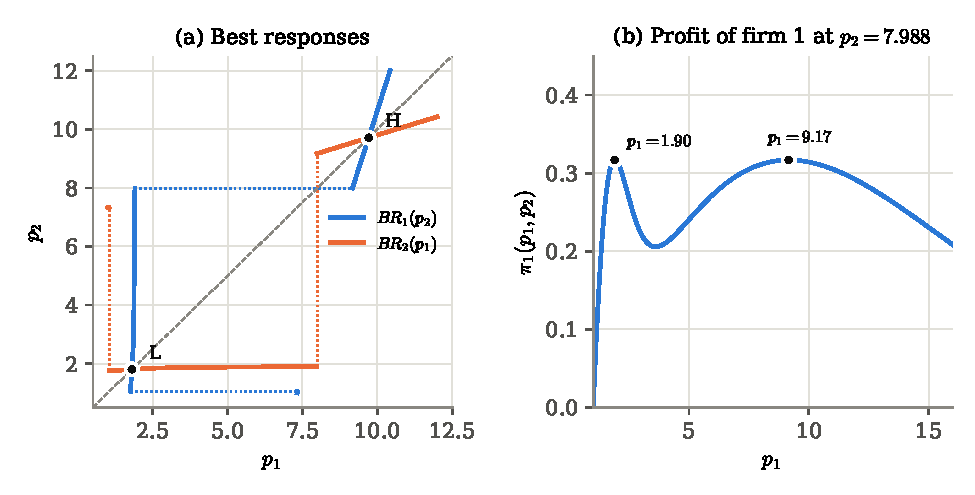
\includegraphics[width=\textwidth]{figures/ch04/multiple_equilibria.pdf}
  \caption{Two equilibria in the two-segment logit duopoly of \cref{ex:04-multiple-eq}. Panel (a): best responses
  $BR_1(p_2)$ and $BR_2(p_1)$, with dotted segments marking the jumps. They cross on the 45-degree line at the
  mass-market equilibrium $L$ ($p^* = 1.804$) and at the niche equilibrium $H$ ($p^* = 9.711$). Panel (b): firm 1's
  profit as a function of its own price when $p_2 = 7.988$. Two local maxima, at $p_1 = 1.904$ and $p_1 = 9.168$,
  give the same profit, so profit is not quasi-concave. Computed with
  \texttt{figures/ch04/src/multiple\_equilibria.py}.}
  \label{fig:04-multiple-eq}
\end{figure}

The example violates the Caplin-Nalebuff conditions in an instructive way. Dividing utility by $\alpha_h$, a consumer
of segment $h$ buys $j$ when $\frac{\delta + \epsilon_{ij} - \epsilon_{i0}}{\alpha_h} - p_j$ is largest. A1 holds
with $g(z) = z$ and money-metric types $\nu_{ij} = \frac{\delta + \epsilon_{ij} - \epsilon_{i0}}{\alpha_h}$. Within a
segment, the vector $(\nu_{i1}, \nu_{i2})$ is a linear transformation of independent extreme value shocks and has a
log-concave density. Across segments, its density is a mixture of a component concentrated near
$\frac{\delta}{\alpha_A} = 1.5$ and a component spread around $\frac{\delta}{\alpha_B} = 15$. The mixture is bimodal.
It is not even quasi-concave, so A2 fails, and profit inherits two peaks from the two groups of consumers.

\casehead{Consequences for empirical work}
Multiplicity does not affect the estimation methods of this chapter. At the estimation stage, prices are data. We
evaluate the first-order conditions at observed prices and invert them for marginal costs as in \eqref{eq:04-mc-recover},
so we never solve for an equilibrium. Whichever equilibrium generated the data, the first-order conditions hold at
the observed prices. In games of entry and in dynamic games, by contrast, multiplicity complicates estimation
itself.

Counterfactuals are different. A merger simulation or a policy experiment must solve for new prices, and with
several solutions the researcher must choose among them. Three selection rules are common. The first starts the
solver at the status quo prices. Merger simulations usually iterate from pre-merger prices, which selects the
equilibrium in whose basin of attraction the status quo lies. The \emph{basin of attraction} of an equilibrium is
the set of starting points from which the iteration converges to it. The second picks the equilibrium the firms prefer,
which here is $H$. The third requires stability under best-response dynamics. In \cref{ex:04-multiple-eq} both
equilibria are stable. Simultaneous best-response iteration from a symmetric start converges to $L$ for starting
prices below 7.988 and to $H$ above. From an asymmetric start such as $(2, 12)$, however, it cycles between
$(1.804, 9.711)$ and $(9.711, 1.804)$, although neither point is an equilibrium. Alternating best responses avoid
the cycle. Stability depends on the adjustment process, and a careful counterfactual reports how its answer depends
on the selection rule (\cref{sec:04-counterfactuals}).

These problems explain part of the popularity of demand systems with known uniqueness results, such as the logit and
CES with multi-product firms (\cref{thm:04-logit-unique} and \citealp{NockeSchutz2018}). For richer systems, the checks
listed at the end of \cref{sec:04-uniqueness} are the practical safeguard. They cannot prove uniqueness, but they can
reveal multiplicity when it is present.
